%% supplement_source.tex
%%
%% RAW MATERIAL FOR THE SUPPLEMENT. This file is not compiled: main.tex does not \input
%% it, it has no preamble, and it does not sync to Overleaf.
%%
%% What it is: the parts of paper/main.tex that left the body on 2026-11-25, moved here
%% word for word, in the order in which they stood in main.tex at commit 3044981. The
%% numbers, labels, citations and generator comments are untouched. Nothing was rewritten.
%%
%% What it holds:
%%   - the Supporting Analyses section, whole (the May sweep task by task, the delivery
%%     gap at the frontier, calling and steering, difficulty, cost, reasoning mode,
%%     contamination);
%%   - the parts of the Methodology that served that section;
%%   - the repair history of the Results (the rerun's parity criterion, the faulty
%%     unaided system message and the second reading, the corrected-prompt control, the
%%     second grading of the lost state traces);
%%   - thinking-on in RQ2 (Table rq2-thinking), the one RQ2 item from the May sweep;
%%   - the Technical Appendix blocks that go with the above.
%%
%% Each block starts with a marker line that says where it stood. Where only some
%% sentences of a paragraph were taken, the marker says so; the rest of that paragraph
%% is still in main.tex. \ref and \label commands point at labels as they were; some of
%% those labels are still in main.tex and some are in this file.
%%
%% Figures used here stay in paper/figures/ (solve.pdf, simulate.pdf,
%% failure_taxonomy.pdf, mechanism_validate_plan.pdf, token_quadrant.pdf). The tables'
%% rows come from the generators named in the comments; the generators and the data stay
%% in the repository.


% ---- from main.tex: Methodology / Tasks, Oracle, and Fixtures, paragraph Test data: the difficulty bins (sentences taken out of the paragraph) ----
% (main.tex at 3044981, from line 556)

The
difficulty bins in
the Supporting Analyses split the trials into thirds. By reference plan length they are at most 8, 9
to 19, and more than 19 steps (on \emph{validate\_plan}, valid plans only). By object
count they are at most 6, 7 to 14, and more than 14 objects (at most 5, 6 to 13, and
more than 13 on \emph{validate\_problem}).


% ---- from main.tex: Methodology / The Three-Arm Design: the fourth (control) arm (end of the last paragraph) ----
% (main.tex at 3044981, from line 765)

A fourth, \emph{control} arm, the steering directive with the tools still
removed, tests whether the directive alone moves the no-tools rate. It serves
only as a control. Its result is reported beside the steering finding (Supporting
Analyses, Table~\ref{tab:ster-units}), and its design and full tables are in the
Technical Appendix.


% ---- from main.tex: Methodology / Metrics, paragraph Storage and what it permits: the run-time grader of the main sweep (one sentence taken out of the paragraph) ----
% (main.tex at 3044981, from line 808)

The unaided arm of the main sweep was graded on the full answer while the
run was in progress, and its rates are exact under that run-time grader
(Supporting Analyses).


% ---- from main.tex: Methodology / Metrics, paragraph Intervals: the Wilson intervals of the Supporting Analyses (one sentence taken out of the paragraph) ----
% (main.tex at 3044981, from line 821)

The Supporting Analyses were computed earlier and
report a Wilson 95\% score interval \citep{wilson1927} for each proportion.


% ---- from main.tex: Methodology / Metrics, paragraph Intervals: the design effect and the model-based checks (rest of the paragraph and the paragraph after it) ----
% (main.tex at 3044981, from line 824)

Each instance is scored
under three paraphrases, so trials within an instance are not independent. The
intraclass correlation is $\approx$0.6 and the design effect $\approx$2.2--2.7, so
the effective sample size is roughly half the nominal count and the Wilson
intervals are correspondingly anti-conservative. We verified that the large
tool-verified gaps of the Supporting Analyses ($+50$--$92$\,pp) and the smallest
gaps reported there remain CI-disjoint after inflating intervals by $\sqrt{2.7}$,
and we flag individually the one gap that does not (the $-5$\,pp
\emph{validate\_problem} steering dip).

As a check on the largest contrast, we also fit an instance-level
random-intercept logistic model to the Gemma-MoE \emph{validate\_plan} comparison
of the plain and the steered arm (tool-verified success $0.206\!\to\!0.926$). The
steering effect is positive and significant (maximum likelihood, log-odds $+7.80$,
SE $0.29$, 95\% interval $[7.23,\,8.37]$). A population-averaged GEE with an
exchangeable working correlation, clustered on domain, estimates a different
quantity and gives $+3.87$ $[2.63,\,5.12]$, with the same sign. The conclusion
therefore does not depend on whether non-independence is handled by design-effect
inflation or by an explicit random-effects model. We do not fit such models cell
by cell, because many cells are near-degenerate or completely separated: the
\emph{simulate} no-tools baseline is $0/3{,}000$ format-exact on the canonical
(shared-budget) corpus, and the tool arms reach
$P(\text{correct}\mid\text{call})\!\approx\!0.99$. A maximum-likelihood GLMM is
undefined or unstable there, whereas the design-effect inflation never fits a
per-cell model and remains valid at the boundary. With cluster size three, the
random-effect variance is also only weakly identified.


% ---- from main.tex: Methodology / Metrics: paragraph Signed significance ----
% (main.tex at 3044981, from line 851)

\paragraph{Signed significance.} The Supporting Analyses use a \emph{signed} rule
for gaps. A per-model gap counts as favorable evidence only when the two arms'
95\% intervals are disjoint and the gap points the hypothesized way (the tool
helps). A disjoint gap that points the other way is counted separately, as
significant \emph{against}. The sign matters. On \emph{validate\_plan}, offering
the tool under the plain prompt leaves one $\geq$9B model calling the validator in
$21\%$ of the trials, and its tool-verified rate is $67$\,pp below its unaided
rate. A test that ignored the sign would count that large movement as the tool
having an effect. The signed rule counts it against the tool at the tool-verified
level, and RQ1 reports what happens to the delivered answer in that cell.
Requiring disjoint 95\% intervals is conservative. It keeps the false-positive
rate well below $\alpha=0.05$ and loses power on small gaps, so a gap that we do
not call significant may still be real. We apply no family-wise correction across
cells, and we treat the few borderline gaps as exploratory.


% ---- from main.tex: Methodology: subsection Comparing Reasoning Modes ----
% (main.tex at 3044981, from line 866)

\subsection{Comparing Reasoning Modes}
\emph{think}~=~off is the mode we report first. The model answers directly, so
the availability and steering gaps measure the tool without interference from the
output budget. Under \emph{think}~=~on the shared decode budget truncates a large
fraction of the $\geq$9B no-tools trials, because the baseline spends its budget
on reasoning. Raw \emph{think}~=~on gaps therefore mix the tool's value with the
collapse of the baseline. We compare the two modes through the difference between
the steered arm and the no-tools arm. We use the steered arm because under
\emph{think}~=~on two of the three $\geq$9B models call the tool less often in
the plain arm (RQ2), so the availability gap would also contain a failure to call
that depends on the mode and that steering repairs. For each model we also report
the smaller of the two modes' differences, which the decode budget of neither
mode can inflate. Where the unaided rate is zero in both modes, as on
format-exact \emph{simulate}, a truncated baseline cannot have inflated the
difference.


% ---- from main.tex: Methodology: subsection Contamination Control ----
% (main.tex at 3044981, from line 882)

\subsection{Contamination Control}
The domains are public, so an unaided baseline could be inflated by
memorization. A separate sweep re-ran the entire matrix on structurally identical
domains with every surface symbol (the names of the domain and of its types,
predicates, functions, actions, constants and objects) renamed to words from an
unrelated theme. The renaming is lexical. Action arities and the precondition and
effect structure are unchanged, so the probe tests memorization of names and does
not test memorization of structure. We pair the two corpora trial by trial and
count a difference as negligible when its $90\%$ interval, clustered by domain or
by problem (whichever is wider), lies inside $\pm5$\,pp, a test chosen after the
sweep. Under \emph{think}~=~off this criterion is met for every model pooled over
the five tasks, and no per-task interval of the $\geq$9B models admits a canonical
advantage of $5$\,pp or more (Supporting Analyses). The data therefore rule out a
memorization advantage of that size on the baseline from which the availability
gap is measured. Under \emph{think}~=~on the criterion is not met for three Qwen
models, with the renamed corpus lower. The clearest cell there traces to
tokenization and not to memory: the renamed prompts ran $\approx$5\% longer, so
more trials were truncated under the shared budget while success given completion
was unchanged.


% ---- from main.tex: Results / RQ1, paragraph Data: the rerun and its registered parity criterion (sentences taken out of the paragraph) ----
% (main.tex at 3044981, from line 935)

The rerun did not meet its registered
parity criterion against the main sweep at the level of whole jobs (Gemma-MoE-26B met
it in $10$ of $10$ cells; the two Qwen models in $15$ of $20$, where $18$ were
required). We therefore treat it as a replication under a separate apparatus: its
figures are never pooled with main-sweep figures and never stand in for them.


% ---- from main.tex: Results / RQ1: paragraph The unaided baseline on solve and simulate ----
% (main.tex at 3044981, from line 1018)

% Every number in this paragraph is generated: tools/reanalysis/control_prompt_fix.py
% (development/NUMBERS.md, block "Corrected-prompt control"). Do not edit a number by hand.
\paragraph{The unaided baseline on \emph{solve} and \emph{simulate}.} In the rerun
the unaided system message of these two tasks asks for a JSON answer by referring to a
schema that the model never received (Limitations), while the user message asks for
parenthesised actions. Most unaided \emph{solve} answers then reason first and give
the plan as JSON in a code block ($198$ to $260$ of the $300$ answers of a model). The
registered grader reads a plan as JSON only when the whole answer is the JSON object,
and otherwise collects every line that has the shape of an action, so for such an
answer it reads no plan or grades the steps of the reasoning together with the plan.
We took two steps. First, we defined a second reading of the answers: on \emph{solve}
the plan in the last code block decides whenever that block holds a plan, and on
\emph{simulate} a trace written as one JSON object per line also counts. Second, we
ran the unaided arm again for the three open-weight models on these two tasks, in a
pre-registered control with three system messages: the registered one, the same
message without the reference to the schema, and a message that states the answer
format in plain words and asks for the final answer in a code block (Technical
Appendix, Prompts). Each cell holds the $300$ trials per task of the rerun, and all
nine cells ran as the tasks of one job. The registration names the format-stated cell as
the unaided baseline and the second reading as the reading quoted for both arms. We
adopted that reading after the answers of the rerun had been seen and before any
answer of the control existed. The tables and figures of \emph{solve} and
\emph{simulate} below follow this rule for the open-weight models. The rerun's own
unaided arm and the registered grade of every cell are the registered record, and the
Technical Appendix gives them (Tables~\ref{tab:rq1-rerun-solve}
to~\ref{tab:control-contrasts}). The tool arms were not run again, so every difference
between a tool arm and this baseline crosses two runs seven weeks apart. The Claude
runs were not part of the control. On \emph{solve} they received the schema that their
message refers to, through the provider's structured-output parameter, and their
unaided rates come from one wording and $100$ trials, so a difference between their
unaided rates and those of the open-weight models is not a comparison of the models.


% ---- from main.tex: Results / RQ1, paragraph State traces against trace length: Gemma-MoE-26B under the format-stated message (end of the paragraph) ----
% (main.tex at 3044981, from line 1133)

For
Gemma-MoE-26B the format-stated message changes how the answers fail on this task.
Asked for a single JSON object, the model wrote one with unbalanced brackets in $47$ of its $300$
answers, and neither reading accepts such an answer. Under the registered message it
mostly wrote one object per line and reached $36.3\%$ over the $300$ trials by the
second reading, against $27.3\%$ with the format stated; the interval of that
difference includes zero. We keep the format-stated cell as its baseline, as
registered.


% ---- from main.tex: Results / RQ1: Table rq1-control and paragraph The tools against the corrected baseline ----
% (main.tex at 3044981, from line 1211)

\begin{table*}[t]
\centering
\footnotesize
\begin{tabular}{@{}llrrr@{}}
\toprule
\textbf{Model} & \textbf{Task} & \textbf{No-tools, format stated (\%)} &
\textbf{+tool, plain (\%)} & \textbf{Difference (points)} \\
\midrule
% rows generated by tools/reanalysis/control_prompt_fix_tex.py (control_prompt_fix_main.tex)
Qwen3.5-9B & \emph{solve} & $42.7$ {\scriptsize$[31.7,\,53.7]$} & $92.0$ {\scriptsize$[85.3,\,97.7]$} & $+49.3$ {\scriptsize$[+36.0,\,+63.0]$} \\
 & \emph{simulate} & $12.7$ {\scriptsize$[6.0,\,20.7]$} & $20.3$ {\scriptsize$[10.3,\,31.3]$} & $+7.7$ {\scriptsize$[-0.7,\,+17.0]$} \\
\addlinespace
Gemma-MoE-26B & \emph{solve} & $54.0$ {\scriptsize$[38.3,\,69.7]$} & $92.3$ {\scriptsize$[87.3,\,97.0]$} & $+38.3$ {\scriptsize$[+23.7,\,+53.7]$} \\
 & \emph{simulate} & $27.3$ {\scriptsize$[15.3,\,40.0]$} & $20.0$ {\scriptsize$[11.3,\,29.7]$} & $-7.3$ {\scriptsize$[-17.0,\,+2.7]$} \\
\addlinespace
Qwen3.6-35B & \emph{solve} & $69.0$ {\scriptsize$[55.0,\,81.3]$} & $78.3$ {\scriptsize$[71.3,\,84.7]$} & $+9.3$ {\scriptsize$[+0.0,\,+19.7]$} \\
 & \emph{simulate} & $33.3$ {\scriptsize$[20.0,\,47.7]$} & $29.3$ {\scriptsize$[17.3,\,42.3]$} & $-4.0$ {\scriptsize$[-11.7,\,+4.3]$} \\
\bottomrule
\end{tabular}
\caption{RQ1, the unaided baseline under a corrected system message (pre-registered
control; \emph{think}=off, $300$ trials per cell). \emph{No-tools, format stated}: the
unaided arm run again with a system message that states the answer format.
\emph{+tool, plain}: the plain tool arm of the rerun. Both arms are read by the second
reading. \emph{Difference}: the tool arm minus the unaided arm over the paired trials;
the two arms come from different runs. The registered grade of every cell is in
Table~\ref{tab:control-cells}. Brackets are 95\% domain-cluster bootstrap intervals.}
\label{tab:rq1-control}
\end{table*}

% Every number in this paragraph is generated: tools/reanalysis/control_prompt_fix.py
% (development/NUMBERS.md, block "Corrected-prompt control"). Do not edit a number by hand.
\paragraph{The tools against the corrected baseline.} Table~\ref{tab:rq1-control}
pairs the plain tool arm with the format-stated cell trial by trial, over all $300$
trials of a model and task. On \emph{solve} the tools are ahead by $49.3$ points for
Qwen3.5-9B and by $38.3$ points for Gemma-MoE-26B. For Qwen3.6-35B the difference is
$+9.3$ points $[+0.0,\,+19.7]$, so the control does not show the tools ahead on
\emph{solve} for that model. On \emph{simulate} the interval of the difference
includes zero for all three models. In the control, the cell with the registered
message is within $4.0$ points of the rerun's unaided rate on both tasks for every
model. The registered criterion for an unchanged setup, an interval within $5$ points,
is met in three of the six cases. It is unresolved for Gemma-MoE-26B on \emph{solve}
and for Qwen3.6-35B on both tasks, where the interval reaches past $5$ points, and by
the registered rule the differences of those three cases are read across a setup that
moved. Removing the reference
to the schema raises the registered grade on \emph{solve} by $14.7$ to $28.3$ points.
Under the second reading the change is $+7.0$, $-6.0$ and $+7.7$ points, so most of
that rise is layout: with the reference the models gave the plan as JSON, which the
registered grader did not read. On \emph{simulate} the reference cost Qwen3.5-9B
$12.7$ points under both readings.


% ---- from main.tex: Results / RQ2: Table rq2-thinking and paragraph Reasoning mode ----
% (main.tex at 3044981, from line 1406)

\begin{table*}[t]
\centering
\footnotesize
\setlength{\tabcolsep}{3.5pt}
\begin{tabular}{@{}llrrrrr@{}}
\toprule
\textbf{Model} & \textbf{Think} & \textbf{\emph{validate\_domain}} & \textbf{\emph{validate\_problem}} &
\textbf{\emph{validate\_plan}} & \textbf{\emph{solve}} & \textbf{\emph{simulate}} \\
\midrule
% rows generated by tools/reanalysis/rq23_tex.py (rq2_thinking.tex)
Qwen3.5-0.8B & off & $98.6$ {\scriptsize$[95.8,\,100.0]$} & $95.3$ {\scriptsize$[89.5,\,99.3]$} & $92.8$ {\scriptsize$[86.7,\,97.7]$} & $54.7$ {\scriptsize$[39.0,\,69.7]$} & $48.3$ {\scriptsize$[36.0,\,60.0]$} \\
 & on & $90.3$ {\scriptsize$[83.9,\,95.6]$} & $94.3$ {\scriptsize$[89.8,\,97.7]$} & $68.6$ {\scriptsize$[57.6,\,79.0]$} & $36.0$ {\scriptsize$[26.3,\,46.0]$} & $32.7$ {\scriptsize$[25.3,\,40.0]$} \\
Qwen3.5-4B & off & $100.0$ {\scriptsize$[100.0,\,100.0]$} & $99.8$ {\scriptsize$[99.5,\,100.0]$} & $99.9$ {\scriptsize$[99.8,\,100.0]$} & $92.0$ {\scriptsize$[83.3,\,98.7]$} & $96.7$ {\scriptsize$[94.3,\,98.7]$} \\
 & on & $100.0$ {\scriptsize$[100.0,\,100.0]$} & $100.0$ {\scriptsize$[100.0,\,100.0]$} & $98.8$ {\scriptsize$[97.9,\,99.5]$} & $78.3$ {\scriptsize$[66.3,\,89.0]$} & $98.3$ {\scriptsize$[97.0,\,99.7]$} \\
Qwen3.5-9B & off & $100.0$ {\scriptsize$[100.0,\,100.0]$} & $100.0$ {\scriptsize$[100.0,\,100.0]$} & $97.9$ {\scriptsize$[94.2,\,100.0]$} & $99.3$ {\scriptsize$[98.0,\,100.0]$} & $80.0$ {\scriptsize$[76.0,\,84.0]$} \\
 & on & $99.4$ {\scriptsize$[98.6,\,100.0]$} & $98.7$ {\scriptsize$[97.3,\,99.7]$} & $69.2$ {\scriptsize$[61.7,\,76.0]$} & $57.0$ {\scriptsize$[45.3,\,68.7]$} & $94.0$ {\scriptsize$[90.0,\,97.3]$} \\
Gemma-MoE-26B & off & $100.0$ {\scriptsize$[100.0,\,100.0]$} & $99.8$ {\scriptsize$[99.5,\,100.0]$} & $20.7$ {\scriptsize$[9.0,\,34.1]$} & $100.0$ {\scriptsize$[100.0,\,100.0]$} & $99.7$ {\scriptsize$[99.0,\,100.0]$} \\
 & on & $52.5$ {\scriptsize$[36.7,\,68.1]$} & $56.0$ {\scriptsize$[43.7,\,68.0]$} & $0.6$ {\scriptsize$[0.0,\,1.5]$} & $23.3$ {\scriptsize$[15.7,\,31.7]$} & $53.3$ {\scriptsize$[45.0,\,61.7]$} \\
Qwen3.6-35B & off & $100.0$ {\scriptsize$[100.0,\,100.0]$} & $98.5$ {\scriptsize$[97.8,\,99.2]$} & $82.9$ {\scriptsize$[73.5,\,91.1]$} & $64.3$ {\scriptsize$[56.3,\,72.3]$} & $76.3$ {\scriptsize$[67.0,\,84.3]$} \\
 & on & $100.0$ {\scriptsize$[100.0,\,100.0]$} & $100.0$ {\scriptsize$[100.0,\,100.0]$} & $99.9$ {\scriptsize$[99.8,\,100.0]$} & $75.0$ {\scriptsize$[62.7,\,86.3]$} & $99.3$ {\scriptsize$[98.3,\,100.0]$} \\
\bottomrule
\end{tabular}
\caption{RQ2, share of trials that called the right tool (\%), main sweep, plain
prompt, with thinking off and on. On \emph{solve} the right tool is the planner that
fits the domain. Brackets are 95\% domain-cluster bootstrap intervals.}
\label{tab:rq2-thinking}
\end{table*}

\paragraph{Reasoning mode.} Of the runs used for this question, only the main sweep
ran with thinking on (Table~\ref{tab:rq2-thinking}). Under the plain prompt, Gemma-MoE-26B calls the right
tool less often on every task once thinking is on: in $0.6\%$ of the
\emph{validate\_plan} trials, and in $23.3\%$ to $56.0\%$ of the trials of the other
four tasks. Qwen3.5-9B falls on \emph{solve} (from $99.3\%$ to $57.0\%$) and on
\emph{validate\_plan} (from $97.9\%$ to $69.2\%$). Qwen3.6-35B does not fall on any
task. Its plain-prompt calling also differs between the main sweep and the rerun, on
\emph{solve} ($64.3\%$ against $82.7\%$) and on \emph{simulate} ($76.3\%$ against
$99.7\%$), so we quote both runs and read its level with care.


% ---- from main.tex: Results / RQ3: the later reading of the lost plans (sentences taken out of the paragraph) ----
% (main.tex at 3044981, from line 1500)

A later reading of the plans whose
content differs, over both prompts, found that $17$ of the $38$ repeat the tool's plan
exactly and then list the goal facts, which our extractor reads as extra steps, and
that $5$ change an action. That reading is post hoc.


% ---- from main.tex: Results / RQ3: Table rq3-regrade and paragraph The lost state traces, graded a second time ----
% (main.tex at 3044981, from line 1564)

\begin{table*}[t]
\centering
\small
\setlength{\tabcolsep}{4pt}
\begin{tabular}{llrcccrrr}
\toprule
& & & \multicolumn{3}{c}{\textbf{Correct traces lost (\%)}} &
\multicolumn{3}{c}{\textbf{Still lost under the line reader}} \\
\cmidrule(lr){4-6}\cmidrule(l){7-9}
\textbf{Model} & \textbf{Prompt} & \textbf{Tool right} & \textbf{Registered} &
\textbf{Line reader} & \textbf{Difference} & \textbf{No room} & \textbf{Step differs} &
\textbf{Other} \\
\midrule
% rows generated by tools/reanalysis/rq3_simulate_regrade.py (rq3_simulate_regrade.tex)
Qwen3.5-9B & plain & $204$ & $74.5$ {\scriptsize$[60.4,\,87.7]$} & $74.5$ {\scriptsize$[60.4,\,87.7]$} & $+0.0$ {\scriptsize$[+0.0,\,+0.0]$} & $106$ & $37$ & $9$ \\
 & steered & $261$ & $81.2$ {\scriptsize$[70.5,\,90.4]$} & $80.5$ {\scriptsize$[69.7,\,89.8]$} & $-0.8$ {\scriptsize$[-1.9,\,+0.0]$} & $132$ & $41$ & $37$ \\
Gemma-MoE-26B & plain & $272$ & $90.8$ {\scriptsize$[85.4,\,95.5]$} & $77.9$ {\scriptsize$[67.5,\,87.4]$} & $-12.9$ {\scriptsize$[-18.6,\,-7.7]$} & $148$ & $38$ & $26$ \\
 & steered & $272$ & $91.2$ {\scriptsize$[86.0,\,95.8]$} & $79.8$ {\scriptsize$[67.6,\,90.3]$} & $-11.4$ {\scriptsize$[-18.8,\,-5.3]$} & $151$ & $35$ & $31$ \\
Qwen3.6-35B & plain & $282$ & $69.9$ {\scriptsize$[56.5,\,82.4]$} & $68.8$ {\scriptsize$[55.3,\,81.4]$} & $-1.1$ {\scriptsize$[-2.2,\,+0.0]$} & $151$ & $35$ & $8$ \\
 & steered & $287$ & $73.2$ {\scriptsize$[61.3,\,84.2]$} & $65.9$ {\scriptsize$[52.0,\,79.1]$} & $-7.3$ {\scriptsize$[-10.9,\,-3.9]$} & $155$ & $33$ & $1$ \\
\bottomrule
\end{tabular}
\caption{RQ3, \emph{simulate} in the rerun, graded a second time (post hoc). \emph{Tool
right}: trials in which the state-transition tool returned the right trace.
\emph{Registered}: the share of those whose final answer is wrong under the registered grader, as in
Table~\ref{tab:rq3-lost}. \emph{Line reader}: the same share when a trace written as one
JSON object per line is read as well; every state must still equal the answer key.
\emph{Difference}: line reader minus registered grader, in points, paired on the same
trials. The last three columns count the answers still lost under the line reader:
the final turn was refused, clipped or empty (\emph{no room}); a trace with the right
number of steps in which at least one step differs from the answer key (\emph{step differs}); and a trace of
another length or no readable trace (\emph{other}). Brackets are 95\% domain-cluster
bootstrap intervals.}
\label{tab:rq3-regrade}
\end{table*}

\paragraph{The lost state traces, graded a second time.} The pilot is small, so we
measured the two properties on the full rerun, at its 16K window
(Table~\ref{tab:rq3-regrade}). This analysis is post hoc and the registered figures of
Table~\ref{tab:rq3-lost} stay the record. Reading a trace written as one JSON object
per line turns $92$ of the $1{,}266$ lost answers into correct ones. The lost share
falls from $69.9$--$91.2\%$ to $65.9$--$80.5\%$. Most of the change is in
Gemma-MoE-26B ($-12.9$ and $-11.4$ points) and in Qwen3.6-35B under the steered prompt
($-7.3$ points), and the other three cells move by at most $1.1$ points. Layout
therefore explains a part of the loss for one model and little for the other two. An
earlier reading of the $244$ \emph{simulate} answers that no fixed rule could assign,
made by two language-model readers with a third reading to settle disagreements, judged
$154$ of them right in content. It includes other layouts than the one the line reader
handles, and with it the lost share is $65.5$--$75.5\%$. The line reader accepts none of
the $90$ answers that reading judged wrong. The two are not independent, because the
readers were shown the line-by-line parse.

Of the $1{,}174$ answers still lost under the line reader, $843$ are final turns with
no room left or with an empty answer. In $219$ answers the trace has the right number of steps and at least one step
differs from the answer key. In $145$ of the $219$ the only difference is in the listed
predicates and matches the conversion described above: a predicate that the tool
reported as false is listed as true, or one it reported as true is left out. In $47$
the numeric values alone differ, and most of these leave the values out. The remaining
$112$ answers hold a trace of another length or no readable trace. The conversion errors
cannot be given as a share of all losses, because an answer with no room left never
reaches the point where the conversion would show. At 16K the largest group is thus the
answers with no room, and the pilot indicates that a larger window removes the empty
answers and still leaves most of these traces lost.


% ---- from main.tex: Section Supporting Analyses, part 1 (opening text and Table howtoread). Figure funnel, which stood here, stays in main.tex with the PlanBench section ----
% (main.tex at 3044981, from line 1628)

\section{Supporting Analyses}
\label{sec:supporting}
The analyses in this section were carried out before the three research questions
were fixed, and they are organized by task. They rest on the main sweep, on the
frontier runs and on separate controls. They cover what the three questions do not
ask: the unaided baseline in the main sweep, calling and the steering sentence,
difficulty, cost, reasoning mode and contamination.

% Study 1 numbers (main sweep: tool-verified, calling, unaided, contamination): the
% frozen values are in development/NUMBERS.md, block "Study 1 — main sweep figures",
% generated by tools/reanalysis/s1_*.py and tools/reanalysis/01-04. Check that block
% before quoting a Study 1 number here.
% The main sweep's open-weight delivered bounds (the e2e overlay, NUMBERS.md block
% "Job 2 — the delivered surface") are retired and are not quoted in this section.
% Frontier delivered numbers: NUMBERS.md, blocks "Frontier e2e" and "Job 2".
Unless stated otherwise, every figure is \emph{think}~=~off on the three $\geq$9B
models. Reasoning mode is treated in the last subsection.

The main sweep supports three kinds of figure for the open-weight models, and all
three are exact. The \emph{unaided} rate is the harness's grade of the model's full
answer, made while the run was in progress. The \emph{calling} rate is the share of
with-tools trials that called the task's tool. The \emph{tool-verified} rate is the
share of with-tools trials in which a tool response held a correct result
(Methodology). Tool calls and their results were stored in full. The final answer
was stored only up to $500$ characters, so the main sweep gives no delivered rate
for its tool arms and we report none. The delivered comparison for the open-weight
models comes from the pre-registered rerun, with the unaided baseline of \emph{solve}
and \emph{simulate} taken from its control, and is reported under RQ1 and RQ3.

The unaided rate of the main sweep also comes from a different grader than the
delivered rates of the rerun. On the same unaided \emph{solve} answers of the rerun,
the run-time grader gives $9.7$--$10.7\%$ and the delivered grader $21.3$--$25.3\%$.
The unaided \emph{solve} and \emph{simulate} figures of RQ1 come from a later control
with a corrected system message and are higher still. Unaided figures in this section
should therefore be compared with one another, and not with the unaided figures of
RQ1.

The frontier runs stored answers up to $16{,}384$ characters, so their delivered
rates are exact on four tasks. On \emph{simulate} some stored answers end before
the trace does, and such a trial cannot be graded. We report these cells as
censoring bounds \cbnd{a}{b}, where $a$ assumes that every ungraded trial failed
and $b$ that every one succeeded. A comparison that involves a bound is asserted
only if it holds at both ends.

The \emph{availability} gap is +tool(plain)~$-$~no-tools and the \emph{steering}
gap is +tool(steered)~$-$~+tool(plain). A gap is called significant when the two
arms' 95\% intervals are disjoint (Methodology). Table~\ref{tab:howtoread} lists,
for each corpus, what was stored and what this section reports from it.
Figure~\ref{fig:funnel} shows, for the with-tools cells, how many trials call the
tool and how many obtain a correct tool result, against the unaided rate as a
reference line. For the frontier models and PlanBench it also shows how many
deliver a correct answer.

\begin{table*}[t]
\centering
\footnotesize
\begin{tabular}{@{}p{0.26\textwidth}p{0.21\textwidth}p{0.18\textwidth}p{0.26\textwidth}@{}}
\toprule
\textbf{Corpus (arms)} & \textbf{Final-answer storage} & \textbf{Reported here} & \textbf{What it supports} \\
\midrule
Open-weight sweeps, canonical $+$ anonymized (no-tools arm) & graded in full at run
time; stored copies are $500$-char snapshots & unaided rate, exact & unaided
baselines; the contamination comparison \\
Open-weight sweeps (tool arms) & $500$-char snapshot; tool calls and results in
full & calling rate and tool-verified rate, exact; no delivered rate & calling,
steering and tool-verified comparisons \\
Frontier runs, Claude Haiku~4.5 $+$ Sonnet~4.6 (both arms) & $16$K snapshot;
no-tools de-censored from raw batch output & delivered rate, exact, except
\emph{simulate} \cbnd{a}{b} & delivered rates with and without tools; delivered
against tool-verified \\
Output-budget probe, frontier (both arms; \emph{simulate}, $n{=}100$ per cell,
the same trials as the canonical cells) & $64{,}000$-token allowance; $256$K-char
storage & delivered rate, exact & the budget component of the delivery gap;
reported beside, never pooled with, the canonical cells \\
Budget-decoupled control (no-tools) & full text & unaided rate, exact & the
unaided-capability question only \\
\bottomrule
\end{tabular}
\caption{What each corpus of this section stored and what is reported from it.
Wilson 95\% intervals print as $[a,\,b]$ and censoring bounds as \cbnd{a}{b}. A
bound is never narrowed by assuming that ungraded trials succeeded. A difference
between a delivered rate and a tool-verified rate is computed only within one
corpus. The delivered comparison for the open-weight models uses the
pre-registered rerun and its control (RQ1 and RQ3), which are not part of this table.}
\label{tab:howtoread}
\end{table*}


% ---- from main.tex: Section Supporting Analyses, part 2 (from Figure solesource to the end of the section) ----
% (main.tex at 3044981, from line 1737)

\begin{figure*}[t]
\centering
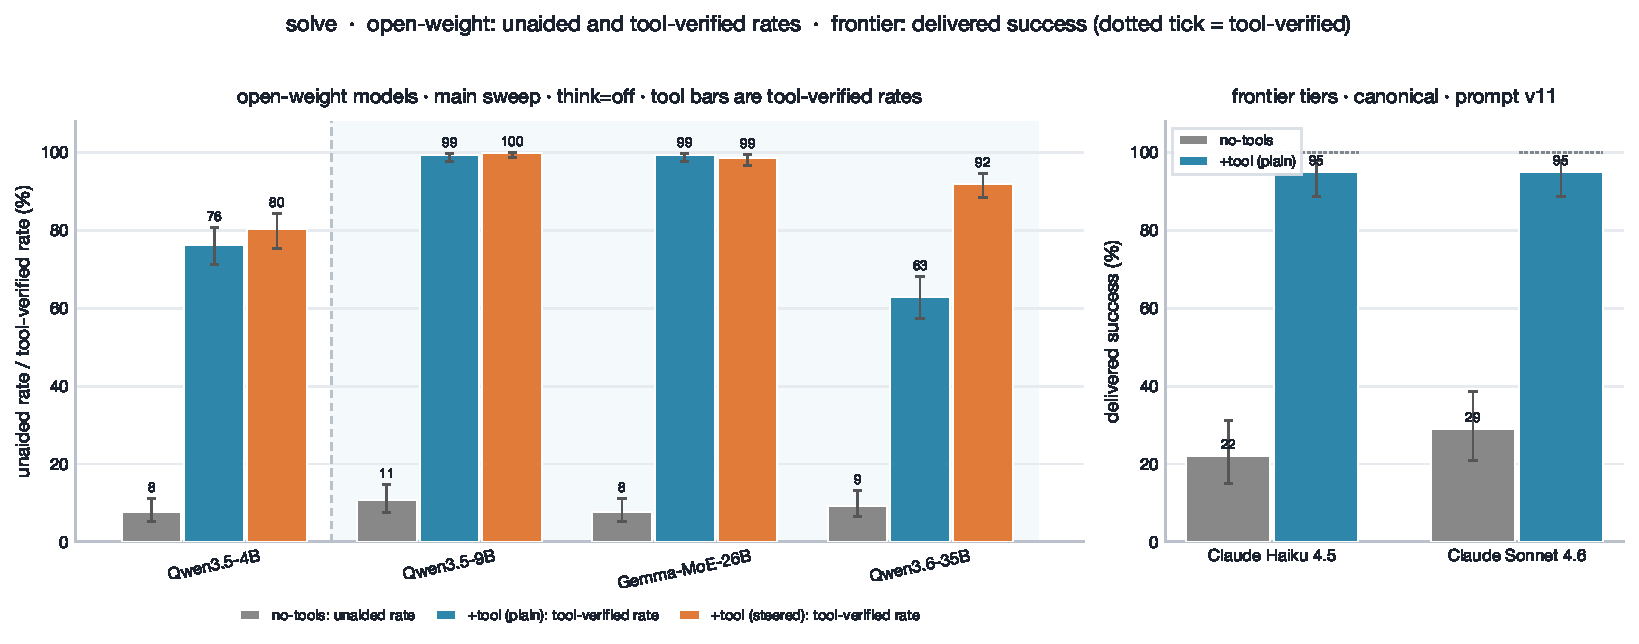
\includegraphics[width=0.49\textwidth]{figures/solve.pdf}\hfill
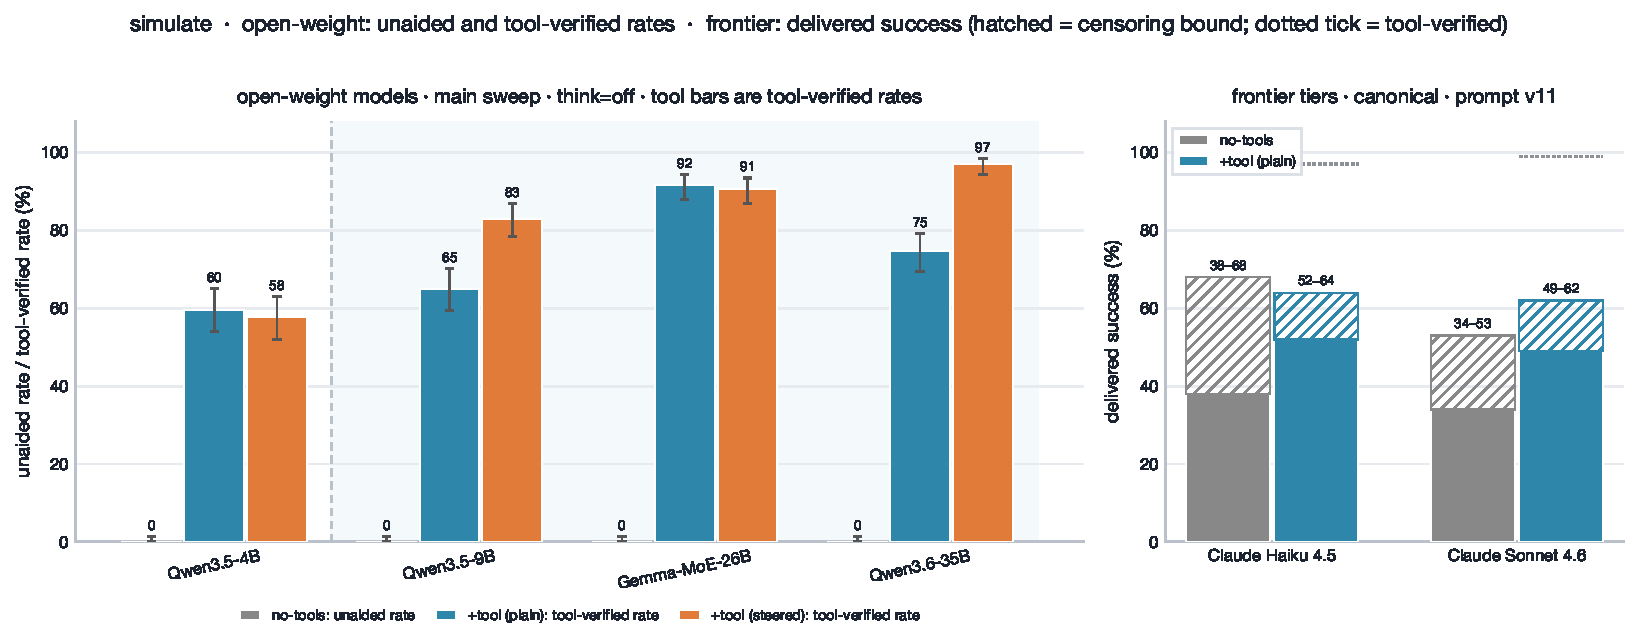
\includegraphics[width=0.49\textwidth]{figures/simulate.pdf}
\caption{\emph{Solve} (left) and \emph{simulate} (right). Whiskers are Wilson 95\%
intervals on exact cells. Frontier panels (prompt v11): the bars are delivered
rates, hatched segments are censoring bounds \cbnd{a}{b}, and the dotted tick
above a tool bar marks the tool-verified rate. On \emph{solve} both models
deliver $95.0\%$ with the tool, against
$22$--$29\%$ unaided and a tool-verified rate of $100\%$. On \emph{simulate} the
delivered bounds are \cbnd{49}{62} (Sonnet) and \cbnd{52}{64} (Haiku) against
unaided \cbnd{34}{53} and \cbnd{38}{68} on the same prompt-v11 slice ($n{=}100$),
and the bounds do not separate the two arms. Open-weight panels (main sweep,
\emph{think}=off; the shaded models are the $\geq$9B ones): the grey bars are the
unaided rates, and the blue and orange bars are the tool-verified rates of the
plain and the steered arm, the share of with-tools trials in which a tool
response held a correct result. The main sweep gives no delivered rate for these
arms; RQ1 and RQ3 report the delivered rates of these models. Unaided
\emph{solve} is $8$--$11\%$ for the shaded models, and the unaided format-exact
rate on \emph{simulate} is $0\%$ for every model.}
\label{fig:solesource}
\end{figure*}

\subsection{\emph{Solve} and \emph{Simulate} in the Main Sweep}
Unaided, the open-weight models rarely pass either task in the main sweep
(Figure~\ref{fig:solesource}). Unaided \emph{solve} is $8$--$11\%$ across the
$\geq$9B models. At the frontier, where storage permits exact delivered rates, the
tool raises Claude Haiku~4.5 from $22\%$ to $95\%$ and Claude Sonnet~4.6 from
$29\%$ to $95\%$. Both differences are CI-disjoint, and both models sit
$5.0$\,pp under their tool-verified rate of $100\%$. The delivery-gap analysis
below takes up those five points. For the open-weight models the delivered
comparison is in RQ1 (Table~\ref{tab:rq1-solve}). What the main sweep adds is the
calling side. The plain-arm tool-verified rates are $63$--$99\%$, and the low end
comes from calling: Qwen3.6-35B calls a planner in $68\%$ of the plain-arm trials,
and steering raises this to $94\%$. In the rerun the same plain-arm cell is
$82.7\%$, so we quote both runs. When a $\geq$9B model does call a planner, the
result is correct in at least $92.6\%$ of the trials, so the tool-verified rate on
\emph{solve} follows the calling rate.

On \emph{simulate} the unaided \emph{format-exact} rate is $0\%$ for every
open-weight model, in both reasoning modes, across all $3{,}000$ trials (a
rule-of-three $95\%$ upper bound of $\leq$0.1\%). The tool returns the correct
trajectory in $65$--$92\%$ of the plain-arm trials and in $83$--$97\%$ of the
steered ones. How much of that reaches the final answer is the subject of RQ3
(Table~\ref{tab:rq3-lost}).

The unaided zero comes from the output budget and the required format. It does
not show that the models cannot track state. Success requires the entire state
trajectory to equal the oracle's under the canonical form, as structured JSON,
with no partial credit and no free-text fallback. The unaided failures of the
$\geq$9B models are $68\%$ unparseable trajectory JSON, $29\%$ answers truncated
at the $6{,}144$-token cap, and $3\%$ answers that parse and are wrong
(Figure~\ref{fig:failtax}). Most answers therefore fail on format or budget before
their content is tested. With the full answers and the delivered grader of the
rerun, the same three models produce $9.9$--$25.5\%$ exact traces unaided
(Table~\ref{tab:rq1-rerun-simulate}). RQ1 reports their unaided traces under a
corrected system message and a second reading (Table~\ref{tab:rq1-simulate}).

A budget-decoupled control separates content from budget. It gives the reasoning
trace and the answer separate decode allowances, through a two-call continuation
that stops decoding at the think-close tag. It was run with \emph{think}=on on the
Qwen models, as a separate corpus that is never pooled with the canonical one, and
it is graded by a wrapper-tolerant grader that scores content and format
separately. Under this control, unaided content-correct state tracking is
$23.0\%$ (4B), $22.3\%$ (9B) and $40.0\%$ (35B), and the $0.8$B model stays at
$0\%$. Re-grading the main corpus's stored responses with the same tolerant grader
recovers at most $0.7\%$. Those responses are $500$-character snapshots, however,
which are too short to regrade (Technical Appendix), so this figure does not
establish how much of the recovery is due to the budget and how much to the
grader. Format compliance stays at $0\%$ for all four models, since none ever
emits the exact requested wrapper, and strict success on content and format
together therefore remains $0\%$. In the matching mode the comparison is
$22$--$40\%$ content-correct unaided against a tool-verified rate of
$87$--$96\%$. The control does not support the claim that these models cannot
track state at all.

\begin{figure*}[t]
\centering
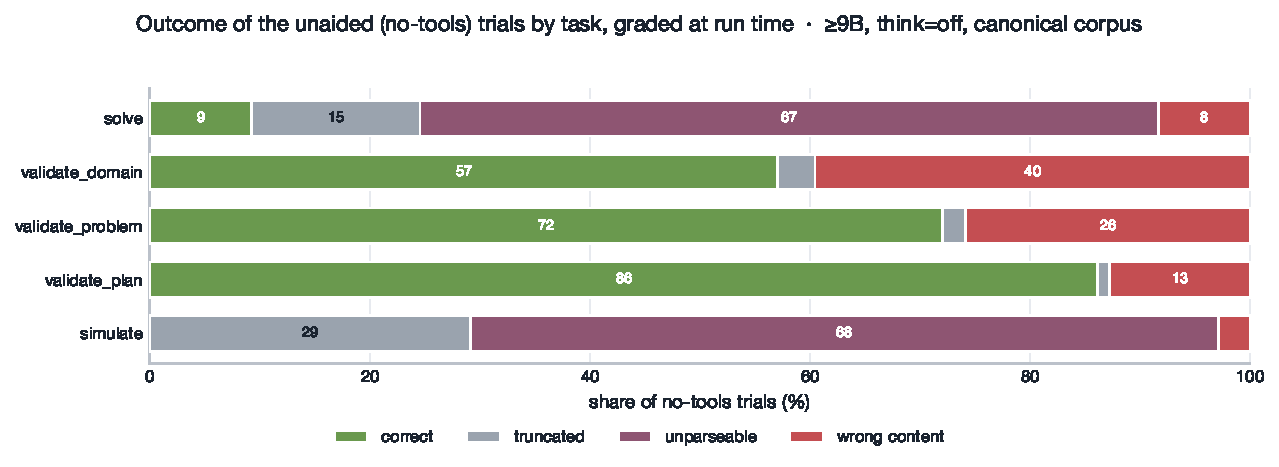
\includegraphics[width=\textwidth]{figures/failure_taxonomy.pdf}
\caption{Outcome of every no-tools trial by task ($\geq$9B, \emph{think}=off,
canonical corpus, pooled), as the harness graded the full answer at run time,
each bar normalized to $100\%$. Every trial is \emph{correct} or exactly one
other outcome: \emph{truncated} (the budget ran out with no answer),
\emph{unparseable}, or \emph{wrong content}. Unaided \emph{solve} is $67\%$
unparseable and $15\%$ truncated, and the unaided validation baselines fail by
wrong content ($13$--$40\%$). Unaided \emph{simulate} is $68\%$ unparseable and
$29\%$ truncated. The tool arms are not drawn, because the main sweep gives no
delivered rate for them. RQ3 reports the loss categories for the tool arms from
the rerun.}
\label{fig:failtax}
\end{figure*}

\subsection{The Delivery Gap at the Frontier}
The frontier with-tools runs let us compare, within one corpus, what the tool
returned with what the model delivered (Table~\ref{tab:deliverygap} and the top
row of Figure~\ref{fig:funnel}). The difference between the tool-verified rate and
the delivered rate is the \emph{delivery gap}. Its pattern is the same for both
models. On the three validation tasks the gap is zero to within a tenth of a
point: a verdict is a short string, and a model that obtains it restates it. On
\emph{solve} both models deliver $95.0\%$ against a tool-verified rate of $100\%$,
a gap of $5.0$\,pp. All five Sonnet failures are trials in which the tool returned
a valid plan and the plan in the final answer does not validate; none is an
omission. Haiku's five are three such plans and two omissions. On \emph{simulate}
the gap is tens of points. The tool returns the correct trajectory in
$97$--$99\%$ of the trials, and the delivered rate is \cbnd{52}{64} (Haiku) and
\cbnd{49}{62} (Sonnet). Half of Sonnet's failures are output budget (trajectories
cut mid-stream or censored at the cap). The rest are split between answers from
which no trajectory can be read and wrong state content.

In these runs the gap grows with the length of what must be restated. A verdict
loses nothing, a plan loses five points, and a trajectory loses a third or more.
The two Claude models do not differ in this: they tie at $95.0\%$ on \emph{solve}
with five failures each, and their \emph{simulate} bounds overlap almost
completely. RQ3 reports the same loss for the open-weight models
(Table~\ref{tab:rq3-lost}). The probe below tests how much of the \emph{simulate}
gap the output budget explains.

\paragraph{Output-budget probe.} Under a pre-registered protocol (Technical
Appendix) we re-ran the same $100$ \emph{simulate} trials per model with the
output allowance raised from $6{,}144$ to $64{,}000$ tokens and the stored
response enlarged from $16$K to $256$K characters, so that no answer is censored.
With the larger allowance, $16/25$ of Sonnet's previously truncated,
budget-fitting failures became correct, compared with $7/19$ of its other failures
re-run under the same apparatus (one-sided Fisher $p=0.069$). This did not meet
the pre-registered confirmation criterion. Haiku met that criterion, with $12/17$
against $1/12$ conversions ($p=0.0011$). None of Haiku's $14$ summary-only
failures, answers that end normally at under a quarter of the trajectory's length,
became correct. Under the 64K output allowance, delivered accuracy with and
without tools was $70\%$ $[60,\,78]$ against $44\%$ $[35,\,54]$ for Sonnet and
$65\%$ $[55,\,74]$ against $58\%$ $[48,\,67]$ for Haiku. Even with the larger
allowance, $30\%$ and $35\%$ of the tool-arm trials failed, and no tool-arm final
response reached the output-token cap. The probe corpus is reported on its own.
The canonical cells and their censoring bounds (\cbnd{49}{62}, \cbnd{52}{64};
Table~\ref{tab:deliverygap}) stand unchanged.

\begin{table}[t]
\centering
\small
\begin{tabular}{@{}lcc@{\hspace{1.2em}}cc@{}}
\toprule
& \multicolumn{2}{c}{\textbf{Haiku 4.5}} & \multicolumn{2}{c}{\textbf{Sonnet 4.6}} \\
\textbf{Task} & \textbf{deliv.} & \textbf{verif.} & \textbf{deliv.} & \textbf{verif.} \\
\midrule
\emph{validate\_domain}  & $98.3$ & $98.3$ & $95.8$ & $95.8$ \\
\emph{validate\_problem} & $96.5$ & $96.5$ & $98.0$ & $98.0$ \\
\emph{validate\_plan}    & $98.8$ & $98.9$ & $100.0$ & $99.9$ \\
\emph{solve}             & $95.0$ & $100.0$ & $95.0$ & $100.0$ \\
\emph{simulate}          & \cbnd{52}{64} & $97.0$ & \cbnd{49}{62} & $99.0$ \\
\bottomrule
\end{tabular}
\caption{The delivery gap at the frontier: delivered success (deliv.) against the
tool-verified rate (verif.), with-tools plain arm, canonical corpus,
\emph{think}=off. $n$ per task: $120$ / $200$ / $1{,}000$ / $100$ / $100$.
Delivered \emph{simulate} cells are censoring bounds ($12$--$13$ of $100$ trials
censored at the $16$K snapshot), and every other cell is exact. The gap is
$\approx$0 on verdicts, $+5.0$\,pp on plans for both models, and $\geq$33\,pp on
trajectories.}
\label{tab:deliverygap}
\end{table}

\subsection{Validating Problems and Domains}
On \emph{validate\_problem} the unaided models are partly competent. The set is
balanced one to one, so a constant ``VALID'' answer scores $\approx$50\%, and the
$\geq$9B models score $65.7$--$75.7\%$ before any tool. With the tool offered
under the plain prompt, the tool-verified rates are $95.2\%$ (9B), $99.7\%$
(Gemma) and $96.8\%$ (35B). In the rerun these models call the validator in at
least $99.3\%$ of the trials (Table~\ref{tab:rq2-choice}) and lose at most $1.7\%$
of its correct verdicts (Table~\ref{tab:rq3-lost}).

\emph{Validate\_domain} behaves differently. Its fixtures run $5{:}1$ valid to
invalid, so a constant ``VALID'' already scores $83\%$. Unaided, every $\geq$9B
model lands at or below that line (pooled $26$--$78\%$), and balanced accuracy
runs from near chance to modest ($53$--$74\%$; Table~\ref{tab:vdom}). Qwen3.5-9B
is the clearest case. It answers ``INVALID'' almost every time (true-positive rate
$12\%$, true-negative rate $95\%$), which gives $26\%$ pooled and $53\%$ balanced.
With the tool under the steered prompt, tool-verified balanced accuracy is
$100.0\%$ (9B), $95.0\%$ (Gemma) and $99.2\%$ (35B), against $53\%$, $74\%$ and
$65\%$ unaided. The Technical Appendix gives the per-class figures.

The 0.8B model behaves differently on the two tasks. On \emph{validate\_domain} its
tool-verified rate under the plain prompt is $87.5\%$, against $80.8\%$ unaided (pooled
rates). On \emph{validate\_problem} it calls the validator in $95.3\%$ of the
plain-prompt trials, yet its tool-verified rate is $26.2\%$, below its unaided $51.2\%$.
In $375$ of those $600$ trials a call to the validator leaves out the required problem
argument. The steered prompt does not repair this: the tool-verified rate is $18.5\%$,
and the argument is missing in $470$ of the $600$ trials.

Steering does not help either validation task at the tool-verified level
($-5$ to ${+}1$\,pp). The one CI-disjoint movement, a $-5$\,pp dip on
\emph{validate\_problem} for the 9B, points against the sentence and does not
survive the paraphrase-clustering correction (Methodology), so we treat it as
non-confirmatory. A capable model that has the tool already calls it, and the
added sentence matters only where the plain arm calls too seldom, as in the next
case.

\begin{figure}[t]
\centering
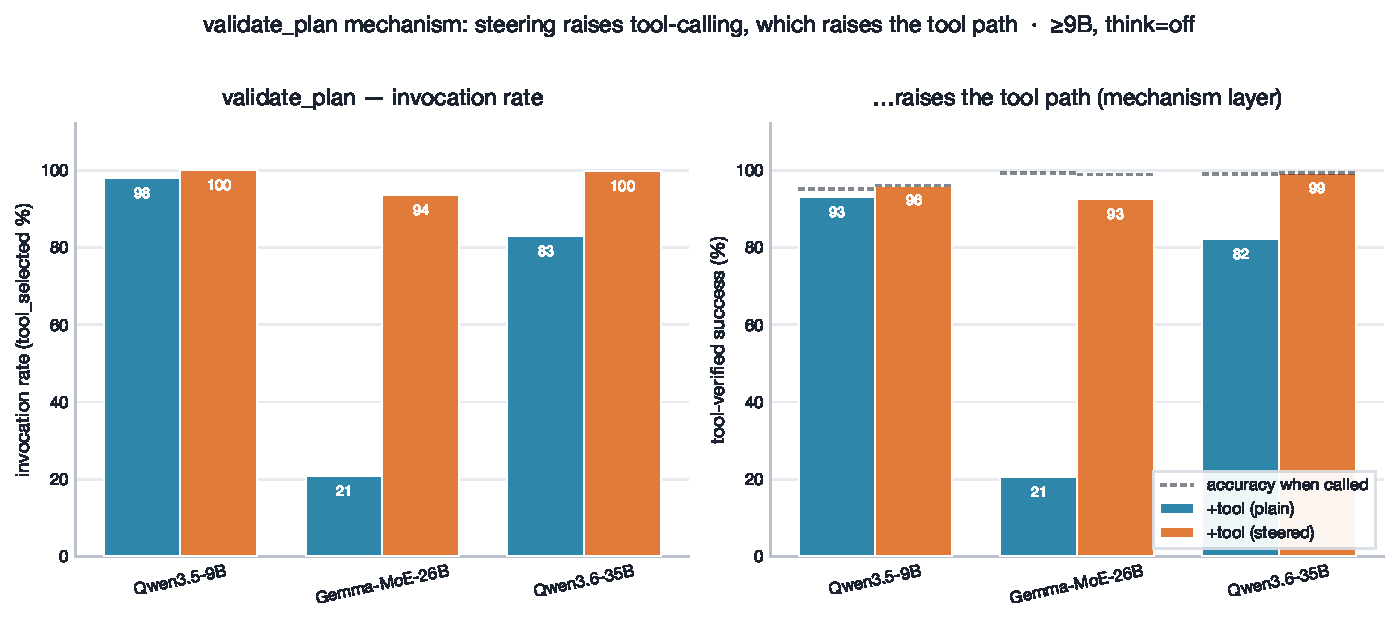
\includegraphics[width=\columnwidth]{figures/mechanism_validate_plan.pdf}
\caption{\emph{Validate\_plan} in the main sweep ($\geq$9B, \emph{think}=off).
Left: calling rate under the plain and the steered prompt. Right: tool-verified
success. Gemma-MoE-26B seldom calls the validator under the plain prompt. The
steering sentence restores calling, and the tool-verified rate rises with it.
Both panels are exact, because tool calls and their results are stored in full.}
\label{fig:mechanism}
\end{figure}

\subsection{\emph{Validate\_plan}: Calling and the Steering Sentence}
\emph{Validate\_plan} is the task the unaided models do best ($\geq$9B no-tools
$80$--$91\%$). It is also the task on which calling varies most.

Under the plain prompt, the tool-verified rate is below the unaided rate for two
of the three $\geq$9B models: $21\%$ against $88\%$ for Gemma-MoE-26B
($-67$\,pp) and $82\%$ against $91\%$ for Qwen3.6-35B ($-9$\,pp). For Qwen3.5-9B
it is above ($93\%$ against $80\%$, $+13$\,pp). These differences set a
tool-verified rate, in which a trial without a call fails by construction, against
the rate of the model's own unaided answers. They describe how the tool was used
and are not a change in the delivered answer. The decomposition shows the cause.
Writing tool-verified success as
$P(\text{call})\times P(\text{correct}\mid\text{call})$, Gemma's low rate is
entirely in the first factor. Under the plain prompt it calls the validator in
$21\%$ of the trials, and when it calls, the result is correct $99\%$ of the
time. Steering moves $P(\text{call})$ from $21\%$ to $94\%$, and the tool-verified
rate follows ($0.94\times0.99=0.93$; Figure~\ref{fig:mechanism}). Across the
$\geq$9B tool cells, $P(\text{correct}\mid\text{call})$ is $95.2\%$ or higher,
with four exceptions: 9B \emph{simulate} ($81.2\%$ plain, $83.3\%$ steered), 9B
\emph{validate\_problem} steered ($90.2\%$), Gemma \emph{simulate} ($92.0\%$ and
$90.7\%$) and 35B \emph{solve} plain ($92.6\%$). Table~\ref{tab:decomp} gives the
cells discussed here. Nearly all the variation in the tool-verified rate between
arms and between models is therefore variation in whether the model calls. These
rates are computed from the stored tool calls and are exact.

The main sweep cannot say whether Gemma's low calling rate lowered its delivered
answers, because it kept only the first $500$ characters of each. The rerun can,
and RQ1 reports it: with the tools offered under the plain prompt, Gemma's verdict
errors stay close to its unaided ones (Table~\ref{tab:rq1-verdicts}). A model that
does not call the validator still answers the question itself, so a low
tool-verified rate does not imply a low rate of correct answers. What the main
sweep establishes is the calling result. Offering the tool changes how often a
model uses it by large amounts that differ between models, and one added sentence
moves Gemma's calling from $21\%$ to $94\%$.

A pre-registered control asks whether that sentence is simply a better prompt.
We appended the same directive to the no-tools prompt, with the tools removed
and the system prompt still stating that they are unavailable, and ran it
beside a neutral-prompt arm in the same job on six (model, mode) units, as a
paired equivalence test at $\pm5$\,pp (Table~\ref{tab:ster-units}; the design and
the full tables are in the Technical Appendix). All six pooled units and all
eight eligible task cells met the $\pm5$\,pp equivalence criterion; excluded
task cells remain unresolved. In the matched cell, Gemma-MoE-26B
\emph{validate\_plan} at \emph{think}=off, the sentence is worth $+72.0$\,pp in
the tool-verified rate with the tool present and $+0.63$\,pp on the model's own
answer with it absent ($90\%$ interval $[-0.46,\,+1.73]$). This supports the
interpretation that steering acts through tool use in the matched Gemma cell.

Calling also explains why the smaller model can look better than the larger one.
In the plain arm the 9B has the higher tool-verified rate (\emph{solve} $99\%$
against $63\%$; \emph{validate\_plan} $93\%$ against $82\%$). The tool-verified
rate follows calling almost one to one, both models are at least $92.6\%$ correct
when they call, and steering closes the gap (35B \emph{solve} from $63\%$ to
$92\%$). The order reverses with reasoning mode: under \emph{think}=on the 35B
calls the validator in $99.9\%$ of the trials and the 9B in $69\%$. The 35B's
unaided baselines exceed the 9B's on every validation task, so the 9B's lead here
reflects how readily each model calls the tool. Two caveats apply. The 35B's
plain-arm calling on \emph{solve} is $68.0\%$ in the main sweep and $82.7\%$ in
the rerun, so we read the direction of this difference and not its size. Our two
largest models are also AWQ-INT4 while the 9B is 16-bit, so this is an observed
difference in calling and not a controlled size effect (Limitations).

\subsection{Plan Length and Object Count}
Both analyses in this subsection set the tool-verified rate of the tool arm
against the unaided rate, bin by bin. RQ1 reports the delivered rates against
plan length and trace length from the rerun and its control. A difference can only be seen to
change where the no-tools baseline has room to move, which makes
\emph{validate\_plan} the informative case. As the reference plan lengthens,
unaided accuracy falls ($94\%$, $91\%$ and $62\%$ over the short, medium and long
bins) while the tool-verified rate holds ($\approx$99\%, $98\%$ and $89\%$), so
the difference widens from $+5$ to $+7$ to $+27$\,pp. On \emph{solve} the
difference is large and roughly constant ($+87$, $+87$ and $+89$\,pp), with the
baseline near its floor and the tool-verified rate near its ceiling. On
\emph{simulate} it is large and declines ($+100$, $+93$ and $+77$\,pp,
CI-disjoint): the baseline stays at a format-exact $0$, and the tool-verified
rate itself falls on long trajectories. Object count moves nothing. The
\emph{validate\_problem} difference is flat at $+22$, $+23$ and $+23$\,pp, and the
other tasks are flat too. The delivered rate behaves differently on \emph{solve}:
with the tools, delivered success falls on the longest plans (RQ1).

\begin{figure*}[t]
\centering
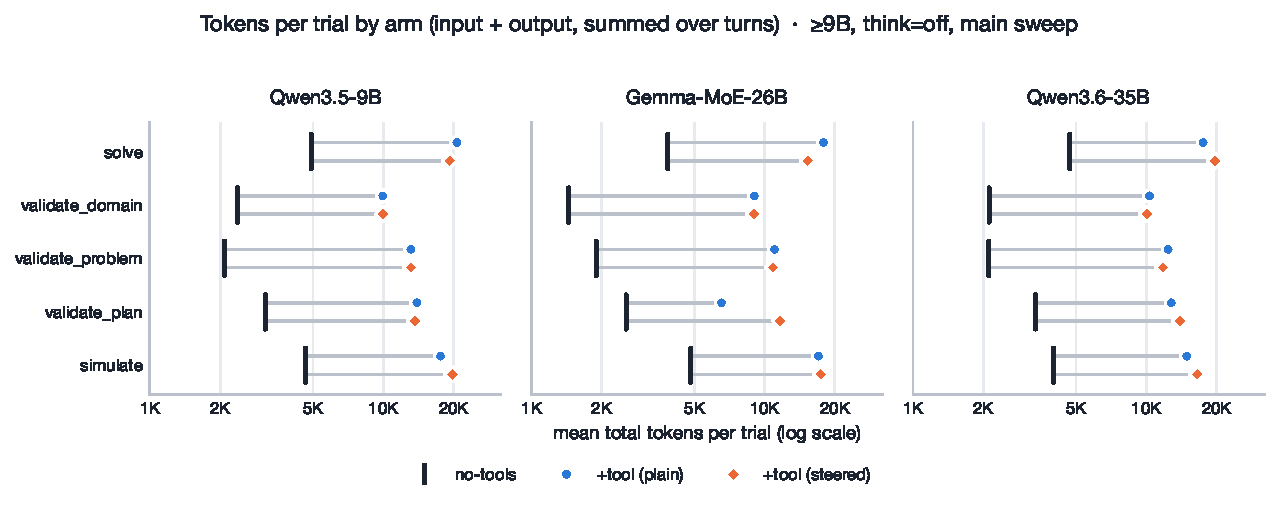
\includegraphics[width=\textwidth]{figures/token_quadrant.pdf}
\caption{Tokens per trial in the main sweep ($\geq$9B, \emph{think}=off), with
one panel per model and one row per task. The horizontal axis is the mean total
tokens per trial (input~$+$~output, summed over turns) on a log scale. In each
row the vertical tick marks the no-tools arm, the circle the plain tool arm and
the diamond the steered tool arm. Both tool-arm markers lie to the right of the
tick in every row: the tool arms always use more tokens per trial.}
\label{fig:tokens}
\end{figure*}

\subsection{What the Tool Costs}
The tool is not free (Figure~\ref{fig:tokens}). Per trial it raises total token
use (input~$+$~output, summed over turns) by $\approx$4--6$\times$ on the
$\geq$9B models and by up to $\approx$15$\times$ on the 4B. The added cost is
input. The unaided model is output-heavy (input:output $\leq$1:1, and as low as
$0.3$:1 on \emph{solve}, where it reasons in the open). The tool arms are
input-heavy ($\approx$6--12:1), because the tool schemas and the tool outputs are
fed back on every turn. Server-side prefix caching, $\approx$90\% on this roster,
makes the re-fed schemas cheap to compute, but tool outputs are not cached and
their tokens still occupy the context. Our totals count all of these tokens raw,
so where caching applies the reported cost of the tool is an over-estimate. A
production system could lower the input overhead further by summarizing or
dropping tool outputs once they have been used. Our harness re-feeds them
verbatim, so the cost-of-pass we report is a worst case and is not tuned for
deployment.

Whether the cost is worth paying depends on the baseline. The choice of metric
changes the verdict by $\approx$10$\times$ on the same data, so we report
\emph{cost-of-pass}, total tokens divided by successful trials (lower is better),
which factors exactly into the tokens-per-trial ratio divided by the success-rate
ratio. For the open-weight models the ratios below count a trial as a success when
the tool returned a correct result, because the main sweep has no delivered rate
for the tool arms. They are therefore not the cost of a delivered answer. Where
the unaided rate is near zero, the tool lowers the cost per success: on
\emph{solve} it is $\approx$0.3--0.4$\times$ the unaided cost (for example,
$\approx$4$\times$ more tokens for $\approx$9--13$\times$ more successes). Where
the unaided rate is already high, the tool raises it: $\approx$3--5$\times$ on
most \emph{validate\_*} cells ($\geq$9B), where the tool is only modestly more
often right and the extra tokens dominate. On \emph{simulate} the unaided arm has
no format-exact success in the main sweep, so its cost per success is undefined
and we report no ratio.

At the frontier the delivered rates are exact, and on \emph{solve} the result is
the opposite. The unaided rate is $22$--$29\%$ and the re-fed context dominates,
so a delivered pass costs $3.1\times$ the unaided tokens for Sonnet ($18.6$K
against $6.0$K) and $6.1\times$ for Haiku ($48.5$K against $8.0$K). On
\emph{simulate} a delivered trajectory costs Sonnet $84$--$106$K tokens against
$10$--$15$K, a premium of $5$--$11\times$.

Cost-of-pass is a ratio of token counts, so it does not depend on the price per
token as long as input and output tokens are priced alike. At representative
commodity serving rates (order \$0.1--\$1 per million tokens) the absolute cost on
the tasks with a near-zero unaided rate is a fraction of a cent per correct
answer. We report token cost and not wall-clock latency, because the batched
server multiplexes trials and per-trial latency cannot be recovered from our
logs. A benchmark at concurrency one would be the right instrument for time.

The output cap also cuts long generations short. Raw rates of hitting the cap are
not comparable across arms, because tool runs have several turns: a cap hit on a
final narration turn does not void the tool's verified result. Trials that hit
the cap and also fail at the tool-verified level stay at $\leq$10\% in the tool
arms, though the same cap hit can cut the final answer (RQ3). We report totals. A
view restricted to completed trials would make the tool look better, and we do
not report it.

\subsection{Reasoning Mode, Contamination and the Frontier Models}
\paragraph{Reasoning mode.} At the tool-verified level, the signed rule applied
to the \emph{think}=on corpus gives the same pattern as under \emph{think}=off.
The raw \emph{think}=on gaps are confounded by the budget, however. Reasoning and
answer share one decode budget ($6{,}144$ tokens; $8{,}192$ for \emph{solve}), and
$14$--$92\%$ of the $\geq$9B no-tools \emph{think}=on trials are truncated
(Gemma-MoE-26B $92\%$, the 35B only $14\%$). This lowers the validation baselines
sharply (\emph{validate\_plan}: 9B from $80\%$ to $21\%$, Gemma from $88\%$ to
$10\%$; \emph{validate\_domain}: Gemma from $78\%$ to $0\%$). We therefore compare
the two modes only through statistics that the budget affects little. The
tool-verified rate of the steered arm is stable across modes (mean shift between
off and on $9$\,pp; the 35B is unchanged on all five tasks), while the no-tools
baseline moves by $28$\,pp, so nearly all the movement across modes is in the
baseline. Taking, for each model, the smaller of the two modes' differences
between the steered arm (tool-verified) and the no-tools arm gives $+46$--$71$\,pp
on \emph{solve} and $+83$--$97$\,pp on \emph{simulate}, where the unaided
format-exact rate is zero in both modes. On the validation tasks the large
\emph{think}=on differences come from the truncated baseline. RQ2 reports calling
under both modes (Table~\ref{tab:rq2-thinking}).

\paragraph{Contamination.} The domains are public, so we re-ran the matrix on
structurally identical domains with all surface names renamed
(Table~\ref{tab:contam}). Paired trial by trial, the \emph{think}=off no-tools
rates of the two corpora meet the $\pm5$\,pp criterion for every model when pooled
over the five tasks (the widest interval is Qwen3.5-4B's, $-2.0$\,pp,
$[-4.3, +0.3]$), so we detect no memorization effect on the unaided baseline. The
pooled rate is dominated by \emph{validate\_plan} ($3{,}000$ of $4{,}560$
trials), so the per-task breakdown (Table~\ref{tab:contam-pertask}) carries more
information. Across the $15$ $\geq$9B (model\,$\times$\,task) cells the mean
$|\Delta|$ is $1.2$\,pp (max $3.7$). The criterion is met in $10$ cells, $6$ of
them at a floor or ceiling where they say little, and not met in $5$
(\emph{validate\_domain} for all three models, \emph{validate\_problem} for
Qwen3.5-9B and Gemma-MoE-26B). In each of those five the renamed corpus scores
higher, the opposite of the direction that memorization of the public domains
would produce, and no per-task interval admits a canonical advantage of $5$\,pp
or more. Under \emph{think}=on the criterion is not met for Qwen3.5-4B,
Qwen3.5-9B and Qwen3.6-35B: pooled, the renamed corpus scores $2.7$ to $4.6$\,pp
lower, the direction memorization would produce. In this mode the shared budget
truncates many trials, and the renamed prompts run $\approx$5\% longer. In
\emph{validate\_plan}, where the two corpora's $95\%$ intervals separate, success
falls $4$--$6$\,pp together with completion while success given completion is
unchanged, so that cell traces to tokenization and not to memory.

\paragraph{A budget-decoupled control.} The shared decode budget confounds the
\emph{think}=on unaided baseline, so we re-ran the unaided arm under the decoupled
apparatus described with the \emph{simulate} results above (separate reasoning
and answer allowances; Qwen models; a separate corpus, never pooled with the
canonical sweep). Beyond the \emph{simulate} recovery reported there
($22$--$40\%$ content-correct at $\geq$4B), the validation baselines rise sharply
(for example \emph{validate\_plan} by $+34$--$60$\,pp for the 4B and the 9B,
Wilson-disjoint). \emph{Solve} is flat for the 9B and the 35B and drops $6$\,pp
at 4B, so decoupling does not help every task. The tool verdicts are unchanged;
what moves is the unaided baseline.

\paragraph{A frontier model without tools.} To test whether these baseline
properties hold beyond the open-weight models, we re-ran the no-tools arm on
Claude Sonnet~4.6 over both corpora at full $N$ (\emph{think}=off;
Table~\ref{tab:frontier}). Its unaided \emph{solve} rate is $28.7\%$, so it
still fails on more than two thirds of the problems without the tool. Its
\emph{simulate} rate is not near zero. After de-censoring from the raw batch
output, the canonical cell is \cbnd{41.7}{61.3} ($59$ of $300$ trials still
indeterminate) and the anonymized cell is \cbnd{36.3}{57.7}. Both lower ends are
far above zero, in line with the budget-decoupled control on the open-weight
models ($22$--$40\%$ at $\geq$4B). Unaided state tracking rises with model
capability once format and budget pressures are removed. The zero of the
open-weight models in the main sweep reflects those pressures ($68\%$
unparseable, $29\%$ truncated; Figure~\ref{fig:failtax}) and does not carry over
to the stronger model.

On contamination the frontier comparison says less than the open-weight one.
Paired trial by trial, the three validation tasks meet the $\pm5$\,pp criterion
(\emph{validate\_domain} $-1.9$\,pp, \emph{validate\_problem} $+0.8$,
\emph{validate\_plan} $+0.0$), but two of them sit at a ceiling. \emph{Solve} is
unresolved. Its totals agree ($28.7\%$ and $28.3\%$), yet its $90\%$ interval,
clustered by domain, is $[-10.6, +9.9]$\,pp, because single domains move in both
directions under renaming (\emph{blocksworld} falls from $11$ to $3$ of $15$
solved answers, \emph{tpp} rises from $0$ to $6$). With one renaming per domain we
cannot tell a memorized domain from a harder renaming, so we report no
memorization effect at the frontier, and no equivalence on \emph{solve} either.
The \emph{simulate} cells are censoring bounds on both corpora and the bounds
overlap broadly, so we claim no drift there. It is the cell that a stronger
contamination design should revisit.

\paragraph{Frontier models with tools.} The frontier corpora also have a
with-tools arm (canonical corpus, wording v11). Their delivered rates are exact,
so the availability gap can be read at the delivered answer. On the validation
tasks the delivered lift is large for Haiku ($+10.8$, $+23.5$ and $+7.3$\,pp on
\emph{validate\_domain}, \emph{validate\_problem} and \emph{validate\_plan}, all
CI-disjoint) and smaller by half to three quarters for Sonnet ($+2.5$, not
separated; $+11.5$; $+2.9$\,pp). On tasks that the model already partly does, the
stronger model leaves the tool less to add. \emph{Solve} is different. The
delivered lift is large for both models ($22\%$ to $95\%$ and $29\%$ to $95\%$),
because the unaided rate barely moves. On \emph{simulate} the with-tools bounds
(\cbnd{49}{62} Sonnet, \cbnd{52}{64} Haiku) are not separated from Sonnet's
unaided \cbnd{41.7}{61.3} at full $N$ (\cbnd{34}{53} on the matching prompt-v11
slice), so we claim no delivered lift there. The tool's work is visible in the
tool-verified rate ($97$--$99\%$) and is lost in delivery, as the delivery-gap
analysis showed. Both frontier models call the tool on essentially every trial,
so the calling results of this section are specific to the open-weight models.

\begin{table}[t]
\centering
\small
\setlength{\tabcolsep}{4pt}
\begin{tabular}{@{}lcccc@{}}
\toprule
\textbf{Model} & \textbf{Canon.} & \textbf{Anon.} & $\Delta$ & \textbf{90\% CI} \\
\midrule
Qwen3.5-0.8B  & 45.9 & 45.8 & $-0.11$ & $[-0.55, +0.34]$ \\
Qwen3.5-4B    & 58.2 & 56.1 & $-2.02$ & $[-4.33, +0.29]$ \\
Qwen3.5-9B    & 63.8 & 64.2 & $+0.35$ & $[-1.52, +2.23]$ \\
Gemma-MoE-26B & 74.3 & 75.2 & $+0.90$ & $[-0.71, +2.51]$ \\
Qwen3.6-35B   & 75.7 & 74.8 & $-0.88$ & $[-2.22, +0.47]$ \\
\bottomrule
\end{tabular}
\caption{Contamination control: no-tools success rate (\%, \emph{think}=off, pooled
over the five tasks) on the canonical and the anonymized-domain corpus, per model
($N=4{,}560$ trials each side). $\Delta=$ anonymized $-$ canonical (pp), paired trial
by trial, with a $90\%$ interval clustered by domain or by problem, whichever is
wider. Every interval lies inside $\pm5$\,pp, so no model shows a detectable
memorization effect at that resolution. The per-task cells, five of fifteen
unresolved, are in Table~\ref{tab:contam-pertask}. The comparison is informative
where the baseline has room to move (e.g.\ Gemma-MoE-26B, Qwen3.6-35B) and
uninformative at the floor.}
\label{tab:contam}
\end{table}

\begin{table}[t]
\centering
\small
\begin{tabular}{@{}lccc@{}}
\toprule
\textbf{Task} & \textbf{Canonical} & \textbf{Anonymized} & $\Delta$ \\
\midrule
\emph{simulate}$^{\S}$           & \cbnd{41.7}{61.3} & \cbnd{36.3}{57.7} & --- \\
\emph{solve}$^\dagger$           & $28.7$ & $28.3$ & $-0.3$ \\
\emph{validate\_problem}         & $89.7$ & $90.5$ & $+0.8$ \\
\emph{validate\_domain}          & $93.6$ & $91.7$ & $-1.9$ \\
\emph{validate\_plan}            & $97.3$ & $97.3$ & $+0.0$ \\
\bottomrule
\end{tabular}
\caption{Claude Sonnet~4.6 without tools: success (\%, \emph{think}=off) on the
canonical and the anonymized-domain corpus, full $N$ per corpus ($300$
\emph{simulate}, $300$ \emph{solve}, $600$ \emph{validate\_problem}, $360$
\emph{validate\_domain}, $3{,}000$ \emph{validate\_plan}; $4{,}560$ each side,
matching Table~\ref{tab:contam}). $\Delta=$ anonymized $-$ canonical, as in
Tables~\ref{tab:contam}--\ref{tab:contam-pertask}, paired trial by trial.
$^\dagger$The \emph{solve} totals agree, but single domains move in both directions
under renaming, so the $90\%$ interval clustered by domain is wide,
$[-10.6, +9.9]$\,pp, and the $\pm5$\,pp criterion is not met. $^{\S}$The
\emph{simulate} cells are censoring bounds \cbnd{a}{b} after de-censoring from raw
batch output ($59$ and $64$ of $300$ trials still indeterminate), so no $\Delta$ is
computed for that row. The three validation tasks meet the criterion
(\emph{validate\_domain} and \emph{validate\_plan} at a ceiling) and the
\emph{simulate} bounds overlap broadly. No memorization effect is detected on the
frontier model, but one is not ruled out on \emph{solve}.}
\label{tab:frontier}
\end{table}


% ---- from main.tex: Technical Appendix: Calling decomposition; Validate_domain per-class accuracy; Per-task contamination; Execution protocol of the output-budget probe; The steering control ----
% (main.tex at 3044981, from line 2726)

\paragraph{Calling decomposition.}
Table~\ref{tab:decomp} gives the decomposition behind the calling results of the
Supporting Analyses. Tool-verified success is factored as
$P(\text{call})\times P(\text{correct}\mid\text{call})$, with
$P(\text{correct}\mid\overline{\text{call}})$ shown where a no-call class exists.
In these rows the spread between arms and between models is almost entirely in
$P(\text{call})$, and accuracy given a call is at least $92.6\%$. Over all
$\geq$9B cells it is $95.2\%$ or higher except in 9B \emph{simulate} ($81.2\%$
plain, $83.3\%$ steered), 9B \emph{validate\_problem} steered ($90.2\%$), Gemma
\emph{simulate} ($92.0\%$ and $90.7\%$) and 35B \emph{solve} plain ($92.6\%$).

\begin{table*}[t]
\centering
\footnotesize
\setlength{\tabcolsep}{4pt}
\begin{tabular}{@{}llcccc@{}}
\toprule
\textbf{Model} & \textbf{Task / arm} & $P(\text{call})$ & $P(\text{c}|\text{call})$ & $P(\text{c}|\overline{\text{call}})$ & \textbf{succ.} \\
\midrule
Gemma-MoE-26B & \emph{val\_plan} plain   & 20.7  & 99.2 & 0.0  & 20.6 \\
Gemma-MoE-26B & \emph{val\_plan} steered & 93.6  & 98.9 & ---  & 92.6 \\
Qwen3.6-35B   & \emph{val\_plan} plain   & 82.9  & 99.1 & 0.0  & 82.2 \\
Qwen3.6-35B   & \emph{val\_plan} steered & 99.9  & 99.4 & ---  & 99.3 \\
Qwen3.5-9B    & \emph{val\_plan} plain   & 97.9  & 95.2 & 0.0  & 93.2 \\
Qwen3.6-35B   & \emph{solve} plain       & 68.0  & 92.6 & 0.0  & 63.0 \\
Qwen3.6-35B   & \emph{solve} steered     & 93.7  & 98.2 & 0.0  & 92.0 \\
\bottomrule
\end{tabular}
\caption{Calling decomposition of tool-verified success (\%, $\geq$9B,
\emph{think}=off, main sweep). The low rate on plain \emph{val\_plan} and its
repair under steering are a change in $P(\text{call})$. Accuracy given a call
($P(\text{c}|\text{call})$) is at least $92.6\%$ in every row. A trial without a
tool call fails this grade by construction, so
$P(\text{c}|\overline{\text{call}})=0$ where it applies (``---'' marks arms with
no no-call class). A model that does not call can still answer correctly itself
(RQ1), so these columns describe the use of the tool and are not the rate of
correct answers.}
\label{tab:decomp}
\end{table*}

\paragraph{\emph{Validate\_domain} per-class accuracy.}
The fixtures run $5{:}1$ valid-to-invalid, so a constant ``VALID'' guess scores
$83.3\%$ pooled but only $50\%$ balanced. Table~\ref{tab:vdom} shows that unaided,
every $\geq$9B model is at or below the pooled trivial line and ranges from near
chance to modest on the balanced metric. We report and test \emph{validate\_domain}
on balanced accuracy, so the metric is the same throughout. With the tool,
tool-verified balanced accuracy rises from $53$--$74\%$ (no-tools) to
$95$--$100\%$, a gap of $+21$--$47$\,pp that is CI-disjoint and favorable for all
three $\geq$9B models. The $60$-trial negative arm widens the balanced interval
but cannot close a gap this large, and the pooled metric yields the same verdict.
Qwen3.5-9B answers ``INVALID'' almost every time (true-positive rate $11.7\%$,
true-negative rate $95.0\%$), which is why its pooled score ($25.6\%$) and its
balanced score ($53.3\%$) differ so much.

\begin{table}[t]
\centering
\footnotesize
\setlength{\tabcolsep}{2.5pt}
\begin{tabular}{@{}lcccc@{}}
\toprule
 & \multicolumn{2}{c}{\textbf{no-tools}} & \multicolumn{2}{c}{\textbf{+tool (steered)}} \\
\cmidrule(lr){2-3}\cmidrule(lr){4-5}
\textbf{Model} & pooled & bal. & pooled & bal. \\
\midrule
Qwen3.5-9B    & 25.6 & 53.3 & 100.0 & 100.0 \\
Gemma-MoE-26B & 77.8 & 74.0 & 98.3  & 95.0  \\
Qwen3.6-35B   & 67.8 & 64.7 & 99.7  & 99.2  \\
\bottomrule
\end{tabular}
\caption{\emph{Validate\_domain} accuracy in the main sweep ($\geq$9B,
\emph{think}=off), pooled (majority-positive) and balanced (per-class mean). The
no-tools columns are the unaided rate and the +tool columns are tool-verified;
both are exact. Trivial baselines are $83.3\%$ pooled and $50\%$ balanced. Unaided
pooled scores are at or below the trivial line and unaided balanced accuracy runs
from near chance to modest.}
\label{tab:vdom}
\end{table}

\paragraph{Per-task contamination.}
Table~\ref{tab:contam-pertask} disaggregates the pooled comparison of
Table~\ref{tab:contam}, which is dominated by \emph{validate\_plan} (3{,}000 of
4{,}560 trials). The $\pm5$\,pp criterion is met in $10$ of the $15$ cells, $6$ of them
at a floor or ceiling (a canonical rate below $10\%$ or above $90\%$), where it carries
little information. It is not met in the $5$ cells marked $^\dagger$, all on
\emph{validate\_domain} or \emph{validate\_problem}. In each of them the anonymized
corpus scores higher, the opposite of the direction memorization of the public
domains would produce, and no interval in the table admits a canonical advantage of
$5$\,pp or more.

\begin{table}[t]
\centering
\footnotesize
\setlength{\tabcolsep}{4pt}
\begin{tabular}{@{}lccccc@{}}
\toprule
\textbf{Model} & \emph{solve} & \emph{v\_dom} & \emph{v\_prob} & \emph{v\_plan} & \emph{sim} \\
\midrule
Qwen3.5-9B    & $+0.7$ & $+1.1^\dagger$ & $+3.7^\dagger$ & $-0.4$ & $+0.0$ \\
Gemma-MoE-26B & $+0.3$ & $+2.8^\dagger$ & $+3.0^\dagger$ & $+0.4$ & $+0.0$ \\
Qwen3.6-35B   & $+0.3$ & $+2.5^\dagger$ & $+1.0$ & $-1.9$ & $+0.0$ \\
\bottomrule
\end{tabular}
\caption{Per-task contamination control: $\Delta=$ anonymized $-$ canonical no-tools
success (pp, \emph{think}=off, $\geq$9B; same sign convention as
Table~\ref{tab:contam}), paired trial by trial. Mean $|\Delta|=1.2$\,pp, max $3.7$,
over $15$ cells. $^\dagger$The $\pm5$\,pp criterion is not met: the $90\%$ interval,
clustered by domain, reaches above $+5$\,pp. In every other cell it is met. The
\emph{sim} column is the format-exact grade, $0\%$ on both corpora.}
\label{tab:contam-pertask}
\end{table}

\paragraph{Execution protocol of the output-budget probe.}
The probe (Supporting Analyses, delivery gap) was pre-registered, and its analysis
code was frozen by hash, before the first API call. For each model we re-ran the
$100$ \emph{simulate} trials of its canonical with-tools cell (the same task,
wording and problem) under the same prompt (v11), temperature~$0$, the same tool
loop (at most ten calls) and the same pinned ground truth. Two settings changed.
The per-turn output allowance was $64{,}000$ tokens for both models, which is
Haiku~4.5's output ceiling, so that the two share one value. The stored response
was $262{,}144$ characters, which no probe answer reached. Each run wrote a manifest of its settings before its first
request, and a resume into a directory whose manifest differed was refused. The
no-tools arms were run at the same allowance through the provider's batch
interface. The primary test is a one-sided Fisher exact test comparing conversion
among the canonical cell's truncated, budget-fitting failures (Sonnet $25$, Haiku
$17$) against its non-truncated failures re-run under the same apparatus (Sonnet
$19$, Haiku $12$), with a confirmation criterion of $p<0.05$ and at least $60\%$
conversion. One infrastructure failure (a Sonnet trial that raised an exception
before producing any tokens) was retried under the runner's existing resume
policy; the completed retry was graded incorrect, and the primary verdicts were
unchanged. No probe answer was censored by storage; no tool-arm final turn reached
the allowance (one Sonnet and two Haiku no-tools answers did). Measured cost of
the four cells was \$40.68.

\paragraph{The steering control.}
The control arm of the Methodology (the steering directive with the tools
removed) was pre-registered as an equivalence test before it was run, after the
main sweeps, in six (model, mode) units: Qwen3.5-4B, Qwen3.5-9B, Gemma-MoE-26B
and Qwen3.6-35B at \emph{think}=off, and the two Qwen models at
\emph{think}=on. Each unit is one job of $9{,}120$ trials: the three neutral
paraphrases of every task (the \emph{anchor}, $4{,}560$ trials) and the same
paraphrases with the directive of Listing~\ref{lst:prompts} appended
($4{,}560$ trials), interleaved by one process against one server, with the
no-tools system prompt unchanged. The \emph{think}=on units use the
budget-decoupled apparatus of the Supporting Analyses with the serving runtime's
reasoning parser off (see the deviations below). The two modes are separate apparatuses,
and no number is compared across them. Gemma-MoE-26B has no \emph{think}=on
unit, because its \emph{think}=on unaided cell saturates the shared decode
budget and the decoupled apparatus relies on a reasoning delimiter that model
does not emit. The hypothesis is that the directive alone moves the no-tools
rate by less than $5$\,pp. The measure is the model's own delivered answer on
determinate rows (rows whose stored answer can be graded). Rows censored at the $16$K storage cap ($1.2$--$1.7\%$ per
unit, all \emph{simulate}) are excluded from every estimator and reported as
bounds. The estimate is the paired difference, steered minus anchor, over
$4{,}466$--$4{,}500$ matched trial pairs per unit, with $90\%$ intervals
clustered on domain ($k{=}20$) and on problem instance (size-weighted, realized
$k{=}220$). The wider interval governs. A unit passes if its pooled interval
lies inside $(-5,\,+5)$ and no eligible task cell has an interval entirely
outside it. The paper-level claim requires every unit to pass, an
intersection-union test that needs no multiplicity correction. A task cell is
eligible when its anchor rate lies in $[10\%,\,90\%]$, its realized
domain-clustered half-width is at most $5$\,pp, and its own paraphrase noise
floor $F$ is below $5$\,pp, where $F$ is the largest absolute difference among
the three designed-null pairs of neutral paraphrases in the anchor arm. A cell
whose $F$ reaches the margin is uninformative at that granularity and cannot
contribute a failure, because the paraphrases alone move it by more than the
effect under test. This gate removes \emph{solve} ($F$ of $14$--$31$\,pp),
\emph{simulate} ($5.6$--$36.3$\,pp) and \emph{validate\_domain}
($5.0$--$14.2$\,pp) in every unit. The registered threshold for declaring a
unit not-equivalent is $5$\,pp plus its realized governing half-width (MDE in
the tables): the smallest $|\hat\Delta|$ at which the interval would lie
entirely outside the margin.

Table~\ref{tab:ster-units} gives the six unit verdicts and
Table~\ref{tab:ster-tasks} every task cell. All six units pass, all eight
eligible task cells meet the $\pm5$\,pp equivalence criterion, and no cell in the family is labeled
not-equivalent. Two pooled intervals (Qwen3.5-9B in both modes) exclude zero on
the positive side while lying inside the margin, which is what the design
treats as floor-equivalent: a real prompt effect below $2$\,pp. The largest
per-task movements (Gemma-MoE-26B \emph{simulate} $+9.0$\,pp at $F{=}36.3$, and
Qwen3.5-9B \emph{think}=on \emph{validate\_domain} $+10.3$\,pp at $F{=}6.7$) sit
in cells the paraphrase gate excluded before the contrast was read and carry
no verdict authority. The matched cell for the body's $+72.0$\,pp,
Gemma-MoE-26B \emph{validate\_plan} at \emph{think}=off, is eligible and
equivalent at $+0.63$\,pp $[-0.46,\,+1.73]$. It contains no censored row.

\begin{table*}[t]
\centering
\footnotesize
\setlength{\tabcolsep}{4pt}
\begin{tabular}{@{}llrrlrrl@{}}
\toprule
\textbf{Model} & \textbf{Mode} & \textbf{Anchor} & \textbf{Steered} & $\hat\Delta$ [90\%] & $F$ & \textbf{MDE} & \textbf{Verdict} \\
\midrule
Qwen3.5-4B & off & 60.3 & 58.8 & $-1.07$ $[-2.32,\,+0.17]$ & 2.09 & 6.25 & pass \\
Qwen3.5-9B & off & 65.6 & 66.7 & $+1.25$ $[+0.01,\,+2.50]$ & 0.55 & 6.25 & pass \\
Qwen3.5-9B & on & 69.7 & 71.7 & $+1.87$ $[+0.69,\,+3.06]$ & 1.67 & 6.18 & pass \\
Gemma-MoE-26B & off & 77.8 & 78.3 & $+0.53$ $[-0.29,\,+1.36]$ & 2.75 & 5.82 & pass \\
Qwen3.6-35B & off & 78.0 & 78.0 & $+0.16$ $[-0.89,\,+1.21]$ & 2.54 & 6.05 & pass \\
Qwen3.6-35B & on & 83.6 & 83.1 & $-0.46$ $[-1.33,\,+0.42]$ & 0.66 & 5.87 & pass \\
\bottomrule
\end{tabular}
\caption{The steering control, unit level (no-tools, \%, delivered answer on
determinate rows). Anchor and steered are the pooled success rates of the two
arms. $\hat\Delta$ is the paired difference, steered minus anchor, with its
governing $90\%$ cluster-robust interval. $F$ is the pooled paraphrase noise
floor of the anchor arm. MDE is the registered threshold for declaring the unit
not-equivalent, $5$\,pp plus the realized half-width. A unit passes when its
interval lies inside $(-5,\,+5)$ and no eligible task cell lies entirely
outside it.}
\label{tab:ster-units}
\end{table*}

\begin{table*}[t]
\centering
\footnotesize
\setlength{\tabcolsep}{4pt}
\begin{tabular}{@{}llrlrrll@{}}
\toprule
\textbf{Unit} & \textbf{Task} & \textbf{Anchor} & $\hat\Delta$ [90\%] & $F$ & \textbf{MDE} & \textbf{Class} & \textbf{Label} \\
\midrule
Qwen3.5-4B (off) & \emph{solve} & 6.7 & $-1.67$ $[-4.32,\,+0.99]$ & 17.00 & 7.65 & uninformative & equivalent \\
 & \emph{val\_domain} & 19.2 & $+0.28$ $[-0.20,\,+0.76]$ & 7.50 & 5.48 & uninformative & equivalent \\
 & \emph{val\_problem} & 56.0 & $-1.00$ $[-3.81,\,+1.81]$ & 5.50 & 7.81 & uninformative & equivalent \\
 & \emph{val\_plan} & 74.5 & {\boldmath $-1.10$ $[-2.86,\,+0.66]$} & 1.40 & 6.76 & eligible & equivalent \\
 & \emph{simulate} & 17.1 & $-2.43$ $[-5.33,\,+0.47]$ & 5.56 & 7.90 & uninformative & unresolved \\
\addlinespace
Qwen3.5-9B (off) & \emph{solve} & 10.3 & $-1.67$ $[-4.89,\,+1.56]$ & 28.00 & 8.23 & uninformative & equivalent \\
 & \emph{val\_domain} & 25.3 & $+4.17$ $[-0.07,\,+8.40]$ & 14.17 & 9.23 & uninformative & unresolved \\
 & \emph{val\_problem} & 66.3 & {\boldmath $+1.33$ $[-1.72,\,+4.39]$} & 4.50 & 8.06 & eligible & equivalent \\
 & \emph{val\_plan} & 79.8 & {\boldmath $+0.63$ $[-1.24,\,+2.50]$} & 1.40 & 6.87 & eligible & equivalent \\
 & \emph{simulate} & 10.9 & $+6.95$ $[+2.71,\,+11.18]$ & 9.78 & 9.24 & uninformative & unresolved \\
\addlinespace
Qwen3.5-9B (on) & \emph{solve} & 26.7 & $+1.33$ $[-4.31,\,+6.98]$ & 16.00 & 10.65 & uninformative & unresolved$^{\dagger}$ \\
 & \emph{val\_domain} & 43.6 & $+10.28$ $[+3.30,\,+17.26]$ & 6.67 & 11.98 & uninformative & unresolved$^{\dagger}$ \\
 & \emph{val\_problem} & 63.8 & $+5.67$ $[+1.76,\,+9.57]$ & 6.50 & 8.90 & uninformative & unresolved \\
 & \emph{val\_plan} & 81.4 & {\boldmath $+0.07$ $[-1.10,\,+1.23]$} & 1.60 & 6.17 & eligible & equivalent \\
 & \emph{simulate} & 32.5 & $+3.83$ $[-3.73,\,+11.39]$ & 30.50 & 12.56 & uninformative & unresolved$^{\dagger}$ \\
\addlinespace
Gemma-MoE-26B (off) & \emph{solve} & 10.3 & $-4.00$ $[-7.68,\,-0.32]$ & 14.00 & 8.68 & uninformative & unresolved \\
 & \emph{val\_domain} & 79.2 & $-1.39$ $[-4.86,\,+2.09]$ & 5.00 & 8.48 & uninformative & equivalent \\
 & \emph{val\_problem} & 77.7 & {\boldmath $-0.50$ $[-2.88,\,+1.88]$} & 4.00 & 7.38 & eligible & equivalent \\
 & \emph{val\_plan} & 88.3 & {\boldmath $+0.63$ $[-0.46,\,+1.73]$} & 2.50 & 6.10 & eligible & equivalent \\
 & \emph{simulate} & 28.0 & $+9.00$ $[+4.68,\,+13.32]$ & 36.33 & 9.32 & uninformative & unresolved \\
\addlinespace
Qwen3.6-35B (off) & \emph{solve} & 10.7 & $-1.33$ $[-5.13,\,+2.46]$ & 31.00 & 8.80 & uninformative & unresolved \\
 & \emph{val\_domain} & 74.4 & $+1.67$ $[-2.14,\,+5.47]$ & 9.17 & 8.80 & uninformative & unresolved \\
 & \emph{val\_problem} & 74.5 & {\boldmath $+0.83$ $[-1.36,\,+3.02]$} & 1.00 & 7.19 & eligible & equivalent \\
 & \emph{val\_plan} & 90.5 & $-0.33$ $[-1.61,\,+0.94]$ & 0.60 & 6.27 & uninformative & equivalent \\
 & \emph{simulate} & 20.7 & $+3.36$ $[-1.01,\,+7.73]$ & 19.26 & 9.37 & uninformative & unresolved \\
\addlinespace
Qwen3.6-35B (on) & \emph{solve} & 42.0 & $-7.67$ $[-14.11,\,-1.23]$ & 26.00 & 11.44 & uninformative & unresolved$^{\dagger}$ \\
 & \emph{val\_domain} & 81.4 & $-2.50$ $[-7.50,\,+2.50]$ & 5.83 & 10.00 & uninformative & unresolved$^{\dagger}$ \\
 & \emph{val\_problem} & 76.0 & {\boldmath $+1.17$ $[-0.36,\,+2.70]$} & 1.50 & 6.53 & eligible & equivalent \\
 & \emph{val\_plan} & 92.6 & $-0.30$ $[-1.10,\,+0.50]$ & 1.20 & 5.80 & uninformative & equivalent \\
 & \emph{simulate} & 45.8 & $+6.32$ $[-0.35,\,+12.98]$ & 16.83 & 11.66 & uninformative & unresolved$^{\dagger}$ \\
\bottomrule
\end{tabular}
\caption{The steering control, every task cell (\%, delivered answer on
determinate rows). Class is assigned mechanically from the anchor arm before
the contrast is read. \emph{Eligible} cells (bold interval) have an anchor rate
in $[10\%,\,90\%]$, a paraphrase floor $F$ below $5$\,pp and a domain-clustered
half-width of at most $5$\,pp. Every other cell is \emph{uninformative} and
carries no verdict authority. An \emph{equivalent} label means the interval lies
inside $(-5,\,+5)$, and \emph{unresolved} means it crosses a margin. No cell
is not-equivalent. MDE is the per-cell threshold for declaring non-equivalence,
as in Table~\ref{tab:ster-units}. $^{\dagger}$ half-width above $5$\,pp
(underpowered).
\emph{Simulate} cells are additionally censoring bounds under extreme
imputation and are reported here on determinate rows only. Their anchor rates
use the delivered grader at $16$K storage and are not comparable to the
format-exact $0\%$ of the Supporting Analyses.}
\label{tab:ster-tasks}
\end{table*}

\emph{Drift check.} The anchor arm doubles as a re-measurement of the canonical
no-tools rates on a later apparatus (Table~\ref{tab:ster-drift}). Pooled over
the four tasks other than \emph{simulate} (whose canonical unaided answers were
stored as $500$-character snapshots and cannot be regraded), the anchor sits at
most $+1.0$\,pp above the canonical corpus, no larger than the $90\%$ sampling
half-width of a single side ($1.0$--$1.2$\,pp at $n{=}4{,}260$ per side per
model). The one per-task movement above $5$\,pp (Qwen3.6-35B
\emph{validate\_domain}, $+6.7$\,pp) is in a cell whose own paraphrase floor is
$9.2$\,pp. This check is reported only here and revises no number elsewhere in
the paper.

\begin{table}[t]
\centering
\footnotesize
\setlength{\tabcolsep}{2.5pt}
\begin{tabular}{@{}lrrrrr@{}}
\toprule
\textbf{Model} & \emph{solve} & \emph{val\_dom.} & \emph{val\_prob.} & \emph{val\_plan} & \textbf{pooled} \\
\midrule
Qwen3.5-4B    & $-1.0$ & $+0.0$ & $-0.5$ & $+0.5$ & $+0.2$ \\
Qwen3.5-9B    & $-0.3$ & $-0.3$ & $+0.7$ & $+0.1$ & $+0.1$ \\
Gemma-MoE-26B & $+2.7$ & $+1.4$ & $+2.8$ & $+0.5$ & $+1.0$ \\
Qwen3.6-35B   & $+1.3$ & $+6.7$ & $-1.2$ & $-0.4$ & $+0.2$ \\
\bottomrule
\end{tabular}
\caption{Drift check: the control's neutral anchor minus the canonical no-tools
rate (pp, \emph{think}=off, $n{=}4{,}260$ per side per model). \emph{Simulate}
is excluded because its canonical unaided answers cannot be regraded.}
\label{tab:ster-drift}
\end{table}

\emph{Within-corpus factorial diagnostic.} The preregistration also fixed an
optional replication check on the two \emph{think}=on units. Their no-tools
legs come from the control run. Their with-tools legs come from an earlier
full-storage rerun of the tool arms with \emph{think}=on, which is a different
corpus from the pre-registered rerun of RQ1 to RQ3 and is used only in this
diagnostic. The two runs share one pinned apparatus.
The estimand is the interaction
$\Delta_{\text{wt}}(\text{steered}-\text{neutral})-
\Delta_{\text{nt}}(\text{steered}-\text{neutral})$ per model, on the delivered
answer for both legs with the same clustered $90\%$ interval, and the
attribution counts as replicated for a model when that interval excludes zero
and its sign matches the model's canonical \emph{think}=on with-tools steering
effect. The replication clause was to enter the main claim only if every model
met the criterion. Fixtures censored on either leg are excluded ($3{,}765$
matched fixtures for Qwen3.5-9B, $4{,}417$ for Qwen3.6-35B). For Qwen3.5-9B
the interaction is $+8.12$\,pp $[+4.61,\,+11.63]$ (with-tools steering
$+8.54$\,pp against no-tools $+1.87$\,pp), and its sign matches the canonical
$+11.38$\,pp, so the criterion is met. For Qwen3.6-35B the interaction is
$+2.62$\,pp $[+0.74,\,+4.50]$ (with-tools $+2.05$\,pp against no-tools
$-0.47$\,pp), but its canonical reference effect is $-0.11$\,pp, an essentially
null reference whose sign cannot meaningfully be matched, so the criterion is
not met. The per-model criterion therefore fails, and the replication clause is
not carried into the main claim, as pre-registered. The diagnostic is bounded
in three ways that the preregistration stated in advance. Gemma-MoE-26B, the
model that owns the $+72.0$\,pp, cannot be in it, because it has no
\emph{think}=on no-tools leg. The factorial is \emph{think}=on while the body's
steering effect is \emph{think}=off, and no \emph{think}=off with-tools steered
corpus was co-run with the control. And the two legs are budget-unmatched by
construction, since the tool loop re-grants the per-task decode budget on every
turn (up to ten calls) while a no-tools trial has one shared budget, so the
comparison was declared attribution-only and no rate from it is quoted as an
effect size. Descriptively, both interactions are positive and exclude zero,
which is consistent with the tool-use reading. On \emph{validate\_plan} alone
the interaction is $+15.0$\,pp $[+9.0,\,+21.0]$ for the 9B and $+2.8$\,pp
$[+0.1,\,+5.4]$ for the 35B, reported because the estimand is stated per model
and a per-task cell carries no clause authority.

\emph{Deviations from the preregistration, declared.} Three changes were made
after the preregistration was ratified. First, the control roster was expanded
from three models to four after interim results were seen. The preregistration
fixed the roster at Qwen3.5-9B, Gemma-MoE-26B and Qwen3.6-35B. With those three
\emph{think}=off units complete and passing, we measured the with-tools steering
effect the control was designed to test across the full roster, in the tool-verified
rate, and found that Qwen3.5-4B carried a larger effect ($+6.9$\,pp pooled,
$+9.6$\,pp on \emph{validate\_plan}) than the controlled Qwen3.5-9B
($+2.5$\,pp), while Qwen3.5-0.8B showed no pooled effect ($+0.0$\,pp) and so
gives the control nothing to test. We added a Qwen3.5-4B \emph{think}=off unit with apparatus
parity to the three completed units. It passes. Under the intersection-union
rule a fourth unit can only make the conjunctive claim harder to satisfy, and
the unit was chosen by the size of its with-tools steering effect, before its
control result was known. Second, the \emph{think}=on arm was rerun with the
reasoning parser off. The preregistration ruled that the parser override is not
passed, reasoning about the single-call path in which reasoning and answer
share one output stream. The \emph{think}=on units use the two-call decoupled
apparatus, and under that rule it produced a void corpus: $9{,}120$ of $9{,}120$
and $3{,}822$ of $3{,}824$ rows with empty answer text, no errors, and about
$13$K tokens generated per row. We cancelled the arm, discarded the void rows
(retained as a failure record), and reran with the parser off, the setting
under which that apparatus had been validated. The rerun reproduces an earlier
parser-off run of the same two models under that apparatus to within a
percentage point on both empty-text share ($8.2\%$ and $3.9\%$ against $8.8\%$
and $4.1\%$ predicted) and success rate ($69.1\%$ and $82.5\%$ against $68.4\%$
and $82.0\%$), and the grading artifact the original rule guarded against does
not appear on this path (unparseable answers are $0.0\%$ on all three
validation tasks in all four affected arms). The two modes were already
declared separate apparatuses whose numbers are never compared, so the change
alters no comparison. Third, after the first readout was ratified, a code
review of the hash-frozen analysis found defects: rows censored at the storage
cap had been scored as delivered successes, the problem-instance
clustering assumed $100$ balanced clusters where the fixture layout yields
$220$ unbalanced ones and so estimated a task-reweighted quantity, and the
secondary mechanism decomposition read fields the graded rows do not carry. The
code was corrected, re-frozen by hash, and the analysis regenerated from the
checkpointed corpus. The corrected analysis preserved all six unit verdicts and
the paper-level branch. The figures reported here are the corrected values.


% ---- from main.tex: Technical Appendix: A pilot with a JSON constraint that takes effect; The rerun's unaided arm on solve and simulate, the registered record; The corrected-prompt control ----
% (main.tex at 3044981, from line 3107)

\paragraph{A pilot with a JSON constraint that takes effect.}
The no-tools arm sent its per-task JSON schema in a request field that the serving
version we used drops, so the schema never reached the decoder (Limitations). Sent in
the field that this version reads, the schema binds. A pilot shows what it then does to
the unaided answers of one model. We ran the $480$ unaided trials of the first problem
of every domain twice for Qwen3.5-9B with thinking off, on the same day: once as the
rerun sent them and once with the schema in the field that binds. The two runs are
paired by trial and graded by the delivered grader of the rerun
(Table~\ref{tab:json-pilot}). With the constraint, $478$ of the $480$ answers begin
with a JSON object. Without it none does. The delivered rate falls by $20.0$ points on
\emph{solve} and by $25.8$ points on \emph{validate\_plan}, where the fall is on the
valid plans ($75.0\%$ to $25.0\%$). On \emph{validate\_domain},
\emph{validate\_problem} and \emph{simulate} the interval of the difference includes
zero. The schema places the verdict before its justification and gives a plan no field
for reasoning, so a constrained answer states its result first, and with thinking off
it has no other place to reason. Constrained \emph{solve} answers are about half as
long ($2{,}159$ against $4{,}078$ tokens on average). We report these two facts beside
the falls and did not test them as their cause. On the validation tasks the prompt of
the constrained run still asks for a closing verdict line. On \emph{solve} and
\emph{simulate} the system message of both runs refers to a schema, which the model
receives in the constrained run alone. The pilot therefore cannot separate the effect
of that reference from the effect of the constraint. The control reported below
measures what the reference did to the unaided answers of the rerun's three models. Between $7$ and $14$
constrained answers per validation task stop at the output cap inside the justification
and so carry no verdict that the grader reads. When the verdict is read from the
opening field of such an answer, the difference on \emph{validate\_domain} becomes
$+9.2$ points $[+2.5,\,+16.7]$, the one on \emph{validate\_problem} becomes $0.0$, and
the one on \emph{validate\_plan} stays at $-25.0$ $[-37.5,\,-12.5]$. The pilot
covers one model and $60$ to $120$ trials per task from $20$ domains, and it was not
registered. A constrained unaided arm is a different condition from the one this paper
reports, and its figures are never set beside the unaided cells of the main sweep or of
the rerun.

\begin{table*}[t]
\centering
\footnotesize
\setlength{\tabcolsep}{5pt}
\begin{tabular}{@{}lrrrr@{}}
\toprule
\textbf{Task} & \textbf{Trials} & \textbf{Prompt only (\%)} & \textbf{Constraint (\%)} &
\textbf{Difference (points)} \\
\midrule
% rows generated by tools/reanalysis/json_constraint_pilot.py (json_constraint_pilot.tex)
\emph{solve} & $60$ & $25.0$ {\scriptsize$[13.3,\,38.3]$} & $5.0$ {\scriptsize$[0.0,\,15.0]$} & ${-}20.0$ {\scriptsize$[{-}31.7,\,{-}10.0]$} \\
\emph{validate\_domain} & $120$ & $50.8$ {\scriptsize$[45.0,\,58.3]$} & $57.5$ {\scriptsize$[49.2,\,66.7]$} & $+6.7$ {\scriptsize$[{-}0.8,\,+14.2]$} \\
\emph{validate\_problem} & $120$ & $56.7$ {\scriptsize$[48.3,\,65.0]$} & $51.7$ {\scriptsize$[41.7,\,61.7]$} & ${-}5.0$ {\scriptsize$[{-}13.3,\,+2.5]$} \\
\emph{validate\_plan} & $120$ & $83.3$ {\scriptsize$[75.8,\,90.0]$} & $57.5$ {\scriptsize$[46.7,\,68.3]$} & ${-}25.8$ {\scriptsize$[{-}39.2,\,{-}13.3]$} \\
\quad valid plans & $60$ & $75.0$ {\scriptsize$[58.3,\,90.0]$} & $25.0$ {\scriptsize$[8.3,\,43.3]$} & ${-}50.0$ {\scriptsize$[{-}68.3,\,{-}30.0]$} \\
\quad broken plans & $60$ & $91.7$ {\scriptsize$[85.0,\,96.7]$} & $90.0$ {\scriptsize$[78.3,\,98.3]$} & ${-}1.7$ {\scriptsize$[{-}15.0,\,+10.0]$} \\
\emph{simulate} & $60$ & $8.3$ {\scriptsize$[1.7,\,16.7]$} & $11.7$ {\scriptsize$[3.3,\,21.7]$} & $+3.3$ {\scriptsize$[{-}5.0,\,+11.7]$} \\
\bottomrule
\end{tabular}
\caption{Pilot: unaided answers of Qwen3.5-9B with the answer format asked for in the
prompt only, as in every unaided cell of this paper, and with a JSON-schema constraint
that takes effect (\emph{think}=off, the first problem of each domain, three wordings,
the same trials in both columns). Entries are delivered rates under the grader of the
rerun. \emph{Difference}: constraint minus prompt only over the paired trials. The
indented rows split \emph{validate\_plan} by whether the plan under test is valid. The
pilot was not registered. Brackets are 95\% domain-cluster bootstrap intervals, not
adjusted for the five tasks.}
\label{tab:json-pilot}
\end{table*}

\paragraph{The rerun's unaided arm on \emph{solve} and \emph{simulate}: the registered record.}
RQ1 reports \emph{solve} and \emph{simulate} for the open-weight models with the
format-stated cell of the control as the unaided baseline and under the second reading.
The registered record of these two tasks is the rerun itself, graded by its registered
delivered grader, with the unaided arm as it was run under the registered system
message. Tables~\ref{tab:rq1-rerun-solve}, \ref{tab:rq1-rerun-simulate}
and~\ref{tab:rq1-rerun-planlen} give it, with the measures of
Tables~\ref{tab:rq1-solve}, \ref{tab:rq1-simulate} and~\ref{tab:rq1-planlen}. The arm
was run again because its system message referred to a schema that never reached the
model (Limitations). Table~\ref{tab:rq1-regrade} applies the second reading to the
rerun's own answers on \emph{solve}, a post hoc analysis made before the control was
run. There the unaided rate rises from $21.3$--$25.3\%$ to $38.3$--$48.0\%$, the rate
with the tools changes by at most $3.3$ points, and the difference between the plain
tool arm and the unaided arm falls from $51.7$--$71.0$ points to $30.3$--$53.7$ points.
No unaided answer of the two Claude models has the layout that the second reading
adds, so their rates are the same under both. The second reading still misses a final
plan that is written as a list in running text below earlier steps. On
\emph{simulate}, reading the rerun's unaided and tool-arm answers with the line reader
moves the difference between the two arms by at most $3.0$ points for any model.

\begin{table*}[t]
\centering
\footnotesize
\setlength{\tabcolsep}{4pt}
\begin{tabular}{@{}llrrrr@{}}
\toprule
& & & \multicolumn{3}{c}{\textbf{Spearman $\boldsymbol{\rho}$ of success with}} \\
\cmidrule(l){4-6}
\textbf{Model} & \textbf{Arm} & \textbf{Solved (\%)} & \textbf{plan length} &
\textbf{object count} & \textbf{planner runtime} \\
\midrule
% rows generated by tools/reanalysis/rq1_tex.py (open-weight rows of rq1_{solve,simulate,planlen}.tex)
Qwen3.5-9B & no-tools & $24.3$ {\scriptsize$[16.3,\,32.3]$} & $-0.29$ & $-0.47$ & $-0.02$ \\
 & +tool (plain) & $88.7$ {\scriptsize$[82.0,\,94.7]$} & $-0.56$ & $-0.08$ & $-0.29$ \\
 & +tool (steered) & $89.0$ {\scriptsize$[82.7,\,94.3]$} & $-0.53$ & $-0.07$ & $-0.21$ \\
\addlinespace
Gemma-MoE-26B & no-tools & $21.3$ {\scriptsize$[13.0,\,30.3]$} & $-0.32$ & $-0.39$ & $-0.11$ \\
 & +tool (plain) & $92.3$ {\scriptsize$[87.3,\,97.0]$} & $-0.44$ & $-0.40$ & $-0.46$ \\
 & +tool (steered) & $95.3$ {\scriptsize$[91.3,\,98.7]$} & $-0.40$ & $-0.13$ & $-0.33$ \\
\addlinespace
Qwen3.6-35B & no-tools & $25.3$ {\scriptsize$[16.3,\,35.7]$} & $-0.34$ & $-0.42$ & $+0.03$ \\
 & +tool (plain) & $77.0$ {\scriptsize$[69.7,\,83.7]$} & $-0.34$ & $-0.30$ & $-0.09$ \\
 & +tool (steered) & $87.3$ {\scriptsize$[81.7,\,92.3]$} & $-0.51$ & $-0.07$ & $-0.30$ \\
\bottomrule
\end{tabular}
\caption{The rerun on \emph{solve}, registered grade (\emph{think}=off, $100$ problems, $300$ trials per row). The no-tools row is the rerun's unaided arm under the registered system message. Columns as in Table~\ref{tab:rq1-solve}. Brackets are 95\% domain-cluster bootstrap intervals.}
\label{tab:rq1-rerun-solve}
\end{table*}

\begin{table*}[t]
\centering
\footnotesize
\setlength{\tabcolsep}{4pt}
\begin{tabular}{@{}llrrrrr@{}}
\toprule
\textbf{Model} & \textbf{Arm} & \textbf{Exact trace (\%)} & \textbf{States, strict (\%)} &
\textbf{States, lenient (\%)} & \textbf{No trace} & $\boldsymbol{\rho}$ \\
\midrule
% rows generated by tools/reanalysis/rq1_tex.py (open-weight rows of rq1_{solve,simulate,planlen}.tex)
Qwen3.5-9B & no-tools & $9.9$ {\scriptsize$[4.2,\,16.7]$} & $18.5$ {\scriptsize$[10.9,\,27.1]$} & $21.7$ {\scriptsize$[14.1,\,30.0]$} & $94$ / $282$ & $-0.52$ \\
 & +tool (plain) & $18.4$ {\scriptsize$[8.9,\,29.1]$} & $24.3$ {\scriptsize$[14.6,\,34.9]$} & $24.7$ {\scriptsize$[14.9,\,35.3]$} & $166$ / $282$ & $-0.55$ \\
 & +tool (steered) & $17.4$ {\scriptsize$[8.9,\,27.4]$} & $22.1$ {\scriptsize$[13.4,\,32.4]$} & $22.4$ {\scriptsize$[13.5,\,32.8]$} & $188$ / $282$ & $-0.58$ \\
\addlinespace
Gemma-MoE-26B & no-tools & $25.5$ {\scriptsize$[14.9,\,36.5]$} & $32.5$ {\scriptsize$[22.0,\,42.9]$} & $36.9$ {\scriptsize$[25.7,\,48.0]$} & $143$ / $282$ & $-0.26$ \\
 & +tool (plain) & $8.9$ {\scriptsize$[4.6,\,14.2]$} & $11.0$ {\scriptsize$[6.6,\,16.1]$} & $12.2$ {\scriptsize$[7.6,\,17.2]$} & $238$ / $282$ & $-0.34$ \\
 & +tool (steered) & $8.9$ {\scriptsize$[4.6,\,13.7]$} & $11.4$ {\scriptsize$[6.6,\,16.7]$} & $12.6$ {\scriptsize$[7.9,\,17.8]$} & $238$ / $282$ & $-0.38$ \\
\addlinespace
Qwen3.6-35B & no-tools & $18.8$ {\scriptsize$[11.2,\,27.3]$} & $24.9$ {\scriptsize$[17.3,\,33.2]$} & $29.5$ {\scriptsize$[21.7,\,37.8]$} & $102$ / $282$ & $-0.23$ \\
 & +tool (plain) & $30.1$ {\scriptsize$[18.1,\,43.7]$} & $36.7$ {\scriptsize$[24.5,\,50.0]$} & $38.5$ {\scriptsize$[26.3,\,51.4]$} & $152$ / $282$ & $-0.73$ \\
 & +tool (steered) & $27.3$ {\scriptsize$[16.5,\,39.4]$} & $33.0$ {\scriptsize$[21.4,\,45.4]$} & $34.1$ {\scriptsize$[22.8,\,46.3]$} & $168$ / $282$ & $-0.70$ \\
\bottomrule
\end{tabular}
\caption{The rerun on \emph{simulate}, registered grade (\emph{think}=off, $94$ problems). The no-tools row is the rerun's unaided arm under the registered system message. Columns as in Table~\ref{tab:rq1-simulate}. Brackets are 95\% domain-cluster bootstrap intervals.}
\label{tab:rq1-rerun-simulate}
\end{table*}

\begin{table*}[t]
\centering
\footnotesize
\setlength{\tabcolsep}{4pt}
\begin{tabular}{@{}llrrrrrrr@{}}
\toprule
\textbf{Model} & \textbf{Arm} & \textbf{Valid plans} & \textbf{Mean len.} &
\textbf{Mean ref.} & \textbf{Median ratio} & \textbf{$<$ / $=$ / $>$ ref.} &
\textbf{Max ratio} & \textbf{$=$ tool's} \\
\midrule
% rows generated by tools/reanalysis/rq1_tex.py (open-weight rows of rq1_{solve,simulate,planlen}.tex)
Qwen3.5-9B & no-tools & $73$ / $300$ & $11.3$ & $13.7$ & $1.00$ & $20$ / $40$ / $13$ & $2.0$ & -- \\
 & +tool (plain) & $266$ / $300$ & $14.9$ & $14.9$ & $1.00$ & $6$ / $252$ / $8$ & $1.1$ & $262$ / $266$ \\
 & +tool (steered) & $267$ / $300$ & $15.4$ & $15.4$ & $1.00$ & $6$ / $253$ / $8$ & $1.1$ & $263$ / $267$ \\
\addlinespace
Gemma-MoE-26B & no-tools & $64$ / $300$ & $9.7$ & $13.0$ & $1.00$ & $15$ / $45$ / $4$ & $1.7$ & -- \\
 & +tool (plain) & $277$ / $300$ & $16.9$ & $16.8$ & $1.00$ & $5$ / $259$ / $13$ & $1.2$ & $269$ / $277$ \\
 & +tool (steered) & $286$ / $300$ & $17.4$ & $17.3$ & $1.00$ & $4$ / $270$ / $12$ & $1.1$ & $280$ / $286$ \\
\addlinespace
Qwen3.6-35B & no-tools & $76$ / $300$ & $11.8$ & $11.1$ & $1.00$ & $15$ / $44$ / $17$ & $3.2$ & -- \\
 & +tool (plain) & $231$ / $300$ & $15.3$ & $15.4$ & $1.00$ & $10$ / $214$ / $7$ & $1.3$ & $213$ / $214$ \\
 & +tool (steered) & $262$ / $300$ & $15.3$ & $15.2$ & $1.00$ & $4$ / $248$ / $10$ & $8.7$ & $257$ / $262$ \\
\bottomrule
\end{tabular}
\caption{The rerun on \emph{solve}, length of the valid delivered plans under the registered grade (\emph{think}=off). Columns as in Table~\ref{tab:rq1-planlen}.}
\label{tab:rq1-rerun-planlen}
\end{table*}

\begin{table*}[t]
\centering
\footnotesize
\setlength{\tabcolsep}{4pt}
\begin{tabular}{@{}lrrrrrr@{}}
\toprule
& \multicolumn{2}{c}{\textbf{No-tools (\%)}} &
\multicolumn{2}{c}{\textbf{+tool, plain (\%)}} &
\multicolumn{2}{c}{\textbf{Difference (points)}} \\
\cmidrule(lr){2-3}\cmidrule(lr){4-5}\cmidrule(l){6-7}
\textbf{Model} & \textbf{Registered} & \textbf{Second reading} & \textbf{Registered} &
\textbf{Second reading} & \textbf{Registered} & \textbf{Second reading} \\
\midrule
% rows generated by tools/reanalysis/rq1_layout_regrade.py (rq1_layout_regrade.tex)
Qwen3.5-9B & $24.3$ {\scriptsize$[16.3,\,32.3]$} & $38.3$ {\scriptsize$[26.3,\,50.3]$} & $88.7$ {\scriptsize$[82.0,\,94.7]$} & $92.0$ {\scriptsize$[85.3,\,97.7]$} & $+64.3$ {\scriptsize$[+54.0,\,+74.7]$} & $+53.7$ {\scriptsize$[+39.0,\,+68.7]$} \\
Gemma-MoE-26B & $21.3$ {\scriptsize$[13.0,\,30.3]$} & $48.0$ {\scriptsize$[32.3,\,63.3]$} & $92.3$ {\scriptsize$[87.3,\,97.0]$} & $92.3$ {\scriptsize$[87.3,\,97.0]$} & $+71.0$ {\scriptsize$[+62.0,\,+79.7]$} & $+44.3$ {\scriptsize$[+30.0,\,+58.7]$} \\
Qwen3.6-35B & $25.3$ {\scriptsize$[16.3,\,35.7]$} & $48.0$ {\scriptsize$[36.3,\,60.0]$} & $77.0$ {\scriptsize$[69.7,\,83.7]$} & $78.3$ {\scriptsize$[71.3,\,84.7]$} & $+51.7$ {\scriptsize$[+42.3,\,+60.0]$} & $+30.3$ {\scriptsize$[+19.3,\,+41.3]$} \\
\bottomrule
\end{tabular}
\caption{RQ1, \emph{solve} in the rerun, graded a second time (post hoc; \emph{think}=off,
$300$ trials per cell). \emph{Registered}: the delivered rate of
Table~\ref{tab:rq1-rerun-solve}. \emph{Second reading}: when the last code block of an answer
holds a plan, that plan is graded in place of the registered reading, whichever way the
grade moves. The same reader is applied to both arms. \emph{Difference}: the plain tool
arm minus the no-tools arm over the paired trials. Brackets are 95\% domain-cluster
bootstrap intervals.}
\label{tab:rq1-regrade}
\end{table*}

% Every number in this paragraph and its two tables is generated:
% tools/reanalysis/control_prompt_fix.py (development/NUMBERS.md, block "Corrected-prompt
% control"); rows by tools/reanalysis/control_prompt_fix_tex.py.
\paragraph{The corrected-prompt control.}
The unaided \emph{solve} and \emph{simulate} system messages of the open-weight runs
refer to a schema that never reached the model (Limitations). The rerun's unaided arm
stays the registered record of those two tasks (Tables~\ref{tab:rq1-rerun-solve}
to~\ref{tab:rq1-rerun-planlen}); the control was run to measure the unaided baseline without
that fault. It covers the three $\geq$9B open-weight models with thinking off and no
tools, on the fixtures, wordings, budgets and serving version of the rerun's unaided
arm. Each model answered the same $300$ trials per task under three system messages
(Prompts): the registered one, the same message with the reference removed, and one
that states the answer format. That gives $5{,}400$ trials. The design, the measures,
the contrasts and the rule that names the format-stated cell as the reported baseline
were registered, and the analysis code was frozen, before any trial ran. No trial
raised an exception and no answer was cut by storage. The serving cluster stopped and
restarted three of the nine cells, twice each, and they resumed from the trials already
written.

Table~\ref{tab:control-cells} gives the rate of every cell under the registered grade
and under the second reading, and Table~\ref{tab:control-contrasts} the paired
contrasts. The registered grade is the delivered grader of the rerun. Under it the
plain tool arm is ahead on \emph{solve} for all three models, by $+55.7$, $+54.7$ and
$+10.7$ points; the last of these does not survive a Holm adjustment over the six
contrasts of its kind. On \emph{simulate} the unaided arm of Gemma-MoE-26B is ahead of
its tool arm by $19.0$ points $[9.0,\,29.7]$. The registered message was run again as a
check on the setup. Its cell differs from the rerun's unaided arm by between $-1.7$ and
$+4.0$ points under either reading. The registered criterion, an interval within $5$
points, is met in three of the six cases and unresolved in the other three, where the
interval reaches past $5$ points. The tool arm was not run again, so the
contrast with the tools crosses two runs seven weeks apart.

One registered check stopped the analysis until it was audited. In the format-stated
cell of Gemma-MoE-26B on \emph{simulate}, $52$ of the $300$ answers end with a final
answer that neither reading accepts. All $52$ give the single JSON object in a code
block that the message asks for. In $47$ the brackets do not balance, and in $5$ the
numeric values are written in a nested form that the grader's trace format does not
have. Both readings count these answers as wrong, and the tool arm is read by the same
parser.

\begin{table*}[t]
\centering
\footnotesize
\begin{tabular}{@{}lllrr@{}}
\toprule
\textbf{Model} & \textbf{Task} & \textbf{System message} &
\textbf{Registered grade (\%)} & \textbf{Second reading (\%)} \\
\midrule
% rows generated by tools/reanalysis/control_prompt_fix_tex.py (control_prompt_fix_cells.tex)
Qwen3.5-9B & \emph{solve} & registered text & $24.3$ {\scriptsize$[16.0,\,33.0]$} & $39.3$ {\scriptsize$[28.0,\,51.0]$} \\
 &  & reference removed & $39.0$ {\scriptsize$[27.3,\,50.7]$} & $46.3$ {\scriptsize$[35.3,\,57.0]$} \\
 &  & format stated & $33.0$ {\scriptsize$[23.0,\,43.0]$} & $42.7$ {\scriptsize$[31.7,\,53.7]$} \\
 & \emph{simulate} & registered text & $7.7$ {\scriptsize$[3.0,\,13.0]$} & $7.7$ {\scriptsize$[3.0,\,13.0]$} \\
 &  & reference removed & $20.3$ {\scriptsize$[11.3,\,30.3]$} & $20.3$ {\scriptsize$[11.3,\,30.3]$} \\
 &  & format stated & $12.7$ {\scriptsize$[6.0,\,20.7]$} & $12.7$ {\scriptsize$[6.0,\,20.7]$} \\
\addlinespace
Gemma-MoE-26B & \emph{solve} & registered text & $22.7$ {\scriptsize$[13.7,\,32.3]$} & $52.0$ {\scriptsize$[37.0,\,66.7]$} \\
 &  & reference removed & $46.0$ {\scriptsize$[31.7,\,60.7]$} & $46.0$ {\scriptsize$[31.7,\,60.7]$} \\
 &  & format stated & $37.7$ {\scriptsize$[26.0,\,49.7]$} & $54.0$ {\scriptsize$[38.3,\,69.7]$} \\
 & \emph{simulate} & registered text & $24.3$ {\scriptsize$[14.0,\,35.0]$} & $36.3$ {\scriptsize$[21.3,\,51.7]$} \\
 &  & reference removed & $18.0$ {\scriptsize$[10.3,\,26.0]$} & $35.7$ {\scriptsize$[21.0,\,51.0]$} \\
 &  & format stated & $27.3$ {\scriptsize$[15.3,\,40.0]$} & $27.3$ {\scriptsize$[15.3,\,40.0]$} \\
\addlinespace
Qwen3.6-35B & \emph{solve} & registered text & $29.3$ {\scriptsize$[19.7,\,39.7]$} & $51.3$ {\scriptsize$[38.0,\,64.7]$} \\
 &  & reference removed & $57.7$ {\scriptsize$[45.3,\,69.0]$} & $59.0$ {\scriptsize$[46.3,\,70.7]$} \\
 &  & format stated & $66.3$ {\scriptsize$[53.0,\,78.3]$} & $69.0$ {\scriptsize$[55.0,\,81.3]$} \\
 & \emph{simulate} & registered text & $19.3$ {\scriptsize$[10.7,\,28.7]$} & $22.7$ {\scriptsize$[13.3,\,33.7]$} \\
 &  & reference removed & $23.7$ {\scriptsize$[12.7,\,35.3]$} & $26.7$ {\scriptsize$[14.3,\,39.7]$} \\
 &  & format stated & $33.3$ {\scriptsize$[20.0,\,47.7]$} & $33.3$ {\scriptsize$[20.0,\,47.7]$} \\
\bottomrule
\end{tabular}
\caption{The corrected-prompt control: share of unaided answers that are right, by
system message (\emph{think}=off, $300$ trials per cell). \emph{Registered text}: the
unaided message of the main sweep and the rerun. \emph{Reference removed}: the same
message without its reference to a schema. \emph{Format stated}: the answer format
given in plain words. Brackets are 95\% domain-cluster bootstrap intervals.}
\label{tab:control-cells}
\end{table*}

\begin{table*}[t]
\centering
\footnotesize
\begin{tabular}{@{}lllrr@{}}
\toprule
\textbf{Contrast} & \textbf{Model} & \textbf{Task} &
\textbf{Registered grade (points)} & \textbf{Second reading (points)} \\
\midrule
% rows generated by tools/reanalysis/control_prompt_fix_tex.py (control_prompt_fix_contrasts.tex)
reference removed minus registered & Qwen3.5-9B & \emph{solve} & $+14.7$ {\scriptsize$[+10.3,\,+19.3]$} & $+7.0$ {\scriptsize$[+0.7,\,+14.7]$} \\
 &  & \emph{simulate} & $+12.7$ {\scriptsize$[+7.0,\,+18.7]$} & $+12.7$ {\scriptsize$[+7.0,\,+18.7]$} \\
 & Gemma-MoE-26B & \emph{solve} & $+23.3$ {\scriptsize$[+12.7,\,+34.3]$} & $-6.0$ {\scriptsize$[-12.0,\,+0.3]$} \\
 &  & \emph{simulate} & $-6.3$ {\scriptsize$[-11.7,\,-1.7]$} & $-0.7$ {\scriptsize$[-3.7,\,+2.7]$} \\
 & Qwen3.6-35B & \emph{solve} & $+28.3$ {\scriptsize$[+20.0,\,+37.0]$} & $+7.7$ {\scriptsize$[+0.0,\,+16.0]$} \\
 &  & \emph{simulate} & $+4.3$ {\scriptsize$[-2.0,\,+10.7]$} & $+4.0$ {\scriptsize$[-3.0,\,+11.3]$} \\
\addlinespace
format stated minus registered & Qwen3.5-9B & \emph{solve} & $+8.7$ {\scriptsize$[+3.7,\,+13.3]$} & $+3.3$ {\scriptsize$[-4.0,\,+11.3]$} \\
 &  & \emph{simulate} & $+5.0$ {\scriptsize$[+1.0,\,+9.0]$} & $+5.0$ {\scriptsize$[+1.0,\,+9.0]$} \\
 & Gemma-MoE-26B & \emph{solve} & $+15.0$ {\scriptsize$[+6.7,\,+23.7]$} & $+2.0$ {\scriptsize$[-3.3,\,+7.3]$} \\
 &  & \emph{simulate} & $+3.0$ {\scriptsize$[-4.7,\,+11.3]$} & $-9.0$ {\scriptsize$[-19.0,\,+1.3]$} \\
 & Qwen3.6-35B & \emph{solve} & $+37.0$ {\scriptsize$[+26.7,\,+48.0]$} & $+17.7$ {\scriptsize$[+7.0,\,+30.3]$} \\
 &  & \emph{simulate} & $+14.0$ {\scriptsize$[+6.0,\,+22.3]$} & $+10.7$ {\scriptsize$[+3.7,\,+18.0]$} \\
\addlinespace
+tool (plain) minus format stated & Qwen3.5-9B & \emph{solve} & $+55.7$ {\scriptsize$[+44.0,\,+67.3]$} & $+49.3$ {\scriptsize$[+36.0,\,+63.0]$} \\
 &  & \emph{simulate} & $+4.7$ {\scriptsize$[-4.0,\,+14.0]$} & $+7.7$ {\scriptsize$[-0.7,\,+17.0]$} \\
 & Gemma-MoE-26B & \emph{solve} & $+54.7$ {\scriptsize$[+43.7,\,+66.3]$} & $+38.3$ {\scriptsize$[+23.7,\,+53.7]$} \\
 &  & \emph{simulate} & $-19.0$ {\scriptsize$[-29.7,\,-9.0]$} & $-7.3$ {\scriptsize$[-17.0,\,+2.7]$} \\
 & Qwen3.6-35B & \emph{solve} & $+10.7$ {\scriptsize$[+1.7,\,+20.7]$} & $+9.3$ {\scriptsize$[+0.0,\,+19.7]$} \\
 &  & \emph{simulate} & $-5.0$ {\scriptsize$[-12.7,\,+3.3]$} & $-4.0$ {\scriptsize$[-11.7,\,+4.3]$} \\
\bottomrule
\end{tabular}
\caption{The corrected-prompt control: paired contrasts over the $300$ trials of a
model and task. The first two blocks compare cells of the control with each other. The
third sets the plain tool arm of the rerun against the format-stated cell and crosses
two runs. Brackets are 95\% domain-cluster bootstrap intervals, not adjusted for the
number of contrasts.}
\label{tab:control-contrasts}
\end{table*}
